%Dokumentklasse
\documentclass[a4paper,12pt]{scrreprt}
\usepackage[left=4cm,right=3cm, bottom=3cm, top=3cm]{geometry}
%\usepackage[onehalfspacing]{setspace}
% ============= Packages =============

% Dokumentinformationen
\usepackage[
	pdftitle={Evaluierung von Elm als Frontend für Webapplikationen},
	pdfsubject={},
	pdfauthor={Philipp Meißner},
	pdfkeywords={},	
	%Links nicht einrahmen
	hidelinks
]{hyperref}


% Standard Packages
\usepackage[utf8]{inputenc}
\usepackage[ngerman]{babel}
\usepackage[T1]{fontenc}
\usepackage{nameref}
\usepackage{graphicx, subfig}
\graphicspath{{img/}}
\usepackage{fancyhdr}
\usepackage{lmodern}
\usepackage{color}
\usepackage{enumitem}
% For inline code
\usepackage{xcolor,listings}

% zusätzliche Schriftzeichen der American Mathematical Society
\usepackage{amsfonts}
\usepackage{amsmath}

%Abkürzungsverzeichnis
%\usepackage[printonlyused,withpage]{acronym}
\usepackage{acronym}

%nicht einrücken nach Absatz
%\setlength{\parindent}{0pt}

% LsListing
% JS:
\lstdefinelanguage{JavaScript}{
  keywords={break, case, catch, continue, debugger, default, delete, do, else, finally, for, function, if, in, instanceof, new, return, switch, this, throw, try, typeof, var, void, while, with},
  morecomment=[l]{//},
  morecomment=[s]{/*}{*/},
  morestring=[b]',
  morestring=[b]",
  sensitive=true
}


% ============= Kopf- und Fußzeile =============
\pagestyle{fancy}
%
\lhead{}
\chead{}
\rhead{\slshape \leftmark}
%%
\lfoot{}
\cfoot{}
\rfoot{\thepage}
%%
\renewcommand{\headrulewidth}{0.4pt}
\renewcommand{\footrulewidth}{0pt}

% ============= Package Einstellungen & Sonstiges ============= 
%Besondere Trennungen
\hyphenation{A-ppli-ka-tion Ja-va-Script}

% ============= Dokumentbeginn =============

\begin{document}
%Seiten ohne Kopf- und Fußzeile sowie Seitenzahl
\pagestyle{empty}

\begin{center}
\begin{tabular}{p{\textwidth}}


\begin{center}
\centerline{
\includegraphics[scale=0.13]{img/logo.png}}
\end{center}


\\

\begin{center}
\LARGE{\textsc{
Evaluierung von Elm als\\ Frontend für Webapplikationen
}}
\end{center}

\\


\begin{center}
\large{Fachhochschule Kiel}
\end{center}

\\

\begin{center}
\textbf{\Large{Bachelor-Thesis}}
%\textbf{\Large{DRAFT}}
\end{center}


\begin{center}
zur Erlangung des akademischen Grades\\
Bachelor of Science
\end{center}


\begin{center}
vorgelegt von
\end{center}

\begin{center}
\large{\textbf{Philipp Meißner}} \\
\small{Matrikelnummer: 922432}
\end{center}


\\

\\\\


\begin{center}
\begin{tabular}{lll}
\textbf{Erstprüfer:} & & Prof. Dr. Robert Manzke\\
\textbf{Zweitprüfer:} & &Prof. Dr. rer. nat. Carsten Meyer\\
\textbf{Abgabetermin:} & & 07.07.2016\\
\end{tabular}
\end{center}

\end{tabular}
\end{center}
\pagenumbering{roman}
\chapter*{Abstract}
\label{sec:Abstract}
Motiviert durch die Versprechungen, die durch die funktionale Programmiersprache Elm gemacht werden \cite[Vgl.]{elm-no-runtime-errors}, ist das Ziel der vorliegenden Bachelor-Thesis, die Programmiersprache, welche in natives JavaScript kompiliert wird, für die Verwendung als Frontend für Webapplikationen anhand einer empirischen Untersuchung zu evaluieren.

Im Zuge dessen wurde eine \acl{SPA} in nativen Elm-Code überführt. Dabei wurde versucht weitestgehend die \acl{CSS}s und \acl{JS}-Dateien beizubehalten. Diese praktische Ausarbeitung wurde anhand unterschiedlichster Bewertungskriterien, wie beispielsweise die Zuverlässigkeit der Applikation, die Performanz einer Elm-Applikation und Portabilität zwischen unterschiedlichen Betriebssystemen und Browsern evaluiert. Ferner wurde die Dateigröße einer minimalen Elm-Applikation ausgewertet und anderen Frameworks gegenübergestellt. Darüber hinaus wurde der erzeugte Quellcode auf Wartbarkeit, Lesbarkeit, und Wiederverwendbarkeit untersucht.

Die praktische Ausarbeitung und Evaluation ergab, dass die Programmiersprache Elm die aufgestellten Kriterien in fast allen Punkten erfüllt. Lediglich die Interoperabilität von bestehenden \ac{JS}-Skripten in eine Elm-Applikation, sowie die Dateigröße einer minimalen Elm-Applikation erwiesen sich als nicht vollständig erfüllt. Die Interoperabilität war dahingehend nicht vollständig funktional, als dass es notwendig war Änderungen an den bestehenden \ac{JS}-Skripten anzufertigen, sowie die nicht praktikable Möglichkeit \ac{CSS}-Dateien nativ in Elm einzubinden. Der Elm-Compiler lieferte keinen Weg die Dateigröße der kompilierten Applikation zu minimieren. Stattdessen musste auf externe Werkzeuge zurückgegriffen werden. Abgesehen davon erwies sich eine Elm-Applikation als sehr performant, effizient und zuverlässig. Zusätzlich gibt es bereits eine Vielzahl an unterstützenden Werkzeugen zur Entwicklung mit Elm.

Die Ergebnisse erlauben die Schlussfolgerung, dass die Entwicklung mit Elm sehr empfehlenswert für Frontend-Entwickler ist. Das Typensystem in Elm erlaubt dem Elm-Compiler eine Vielzahl an Fehlern vorab zu finden. Ferner ist es für einen Entwickler nicht weiter notwendig die erzeugte Elm-Applikation auf allen Browsern separat testen zu müssen, da der Elm-Compiler die Applikation in natives \ac{JS} kompiliert, welches kompatibel mit dem ECMAScript-Standard ist. Daraus entsteht eine enorme Zeitersparnis, die gepaart mit einer effizienten Applikation und einem zuverlässigen Compiler einen deutlich positiven Eindruck von Elm hinterlässt.
\pagenumbering{arabic}
% Beendet eine Seite und erzwingt auf den nachfolgenden Seiten die Ausgabe aller Gleitobjekte (z.B. Abbildungen), die bislang definiert, aber noch nicht ausgegeben wurden. Dieser Befehl fügt, falls nötig, eine leere Seite ein, sodaß die nächste Seite nach den Gleitobjekten eine ungerade Seitennummer hat. 
\cleardoubleoddpage
\pagestyle{fancy}

%Inhaltsverzeichnis
\tableofcontents

\chapter*{Abkürzungsverzeichnis}
\label{sec:Abkürzungsverzeichnis}


%Abkürzungsverzeichnis
%\section{Abkürzungsverzeichnis}
\begin{acronym}[HTML ]
 \acro{SPA}{Single Page Application}
 \acro{HTML}{HyperText Markup Language}
 \acro{DOM}{Document Object Model}
 \acro{CSS}{Cascading Style Sheet}
 \acro{JS}{JavaScript}
 \acro{ID}{Identifier}
 \acro{NPM}{Node Package Manager}
 \acro{URL}{Uniform Resource Locator}
 \acro{APP}{Applikation}
 \acro{HTTP}{Hypertext Transfer Protocol}
 \acro{MVU}{Model-View-Update}
 \acro{Bzw}{Beziehungsweise}
 \acro{IDE}{Integrated Development Environment}
\end{acronym}

%Verzeichnis aller Bilder
\listoffigures

%Verzeichnis aller Tabellen
\listoftables

% pagestyle für gesamtes Dokument aktivieren
\pagestyle{plain}

\chapter{Einleitung}
\label{sec:einleitung}
Die heutige Welt ist sehr schnelllebig und spielt sich immer mehr im Internet ab. Firmen präsentieren sich auf ihren Webseiten und akquirieren dadurch Neukunden. Ganze Geschäfte leben nur noch durch den Online-Handel und besitzen keinerlei Verkaufsläden, in denen ein Kunde das Produkt vorab in den Händen halten kann. Umso wichtiger ist es, das Produkt auf der Webseite außergewöhnlich gut zu präsentieren, um den Kunden zu überzeugen. Webseiten dieser und im Grunde jeglicher Art zielen immer darauf ab, einem Nutzer Informationen bereitzustellen und entsprechend angenehm zu präsentieren. Doch die Entwicklung solcher Systeme ist komplex und geht weit über das Design hinaus. Folglich ist ein großer Teil der Ausgaben von Firmen, die sich online präsentieren, die Bezahlung von Entwicklern für ihre Webapplikationen. Dies können simple Webseiten ohne großartige Funktionen sein, jedoch auch komplexe Systeme wie ein automatisierter Online-Handel, in dem die Nutzer ihren gesamten Einkauf abwickeln können, mitsamt Bezahlung. Demzufolge ist es für die Firmen von großem Interesse, dass die angestellten Entwickler zügig Ergebnisse in der Entwicklung der Webapplikationen machen. Damit der Entwickler effektiv arbeiten kann, braucht er Systeme, die ihn unterstützen. Angefangen bei den Werkzeugen wie seiner Entwicklungsumgebung, bis hin zur tatsächlichen Programmiersprache. Diese wissenschaftliche Arbeit befasst sich mit der neuen Programmiersprache Elm, welche eine funktionale, den deklarativen Programmierparadigmen folgende, Programmiersprache ist. Sie wurde zu Beginn ihrer Entwicklung für die Erstellung von grafischen Benutzeroberflächen und der Verbildlichung mathematischer Funktionen genutzt, bewegt sich nun jedoch immer weiter in Richtung der Webentwicklung und kommt mit einigen Neuheiten, Veränderungen und einer aktiven Gemeinschaft an Open-Source Entwicklern.

Elm verspricht eine blitzschnelle Darstellung von Inhalten selbst bei riesigen Datenmengen mit Hilfe einer Technik die $virtual-dom$ genannt wird. Auch soll es keinerlei Laufzeitfehler mehr geben, da die gesamte Sprache mit Garantien ausgeschmückt ist, die im Zusammenspiel mit dem eigens entwickelten Compiler alle möglichen Fehler vorab findet und darauf hinweist.
All diese Versprechungen werden anhand mehrerer Bewertungskriterien während einer empirischen Entwicklung einer Webapplikation geprüft.

\chapter{Theoretische Grundlagen}
\label{sec:grundlagen}
\pagestyle{plain}

\section{Funktionale Programmiersprachen}
\label{sec:funktionaleProgrammiersprache}
In der Programmierung gibt es zwei Programmierparadigmen, die zur Kategorisierung von Programmiersprachen dienen und sich im Laufe der Zeit entwickelt haben. %„https://de.wikipedia.org/wiki/Programmiersprache#Programmierparadigmen“)
Dabei beschreiben die Paradigmen verschiedene Prinzipien der Programmierung.
Die zugrunde liegenden Kategorien werden häufig als imperative und deklarative Programmierung bezeichnet, in welchen sich jede Programmiersprache einordnen lässt. Jede Kategorie birgt weitere Unterkategorien und dient der Verfeinerung der Prinzipien.
\begin{figure}[h]
\begin{lstlisting}[language=JavaScript]
iterative_function(n) {
  sum = 0;
  for(i = 0; i <= n; i++) {
    sum += i;
  }
}
console.log(iterative_function(10)); // => 55
\end{lstlisting}
\caption{Eine iterative Funktion}\label{fig:iterative-function}
\end{figure}
Häufig gehören funktionale Programmiersprachen dem deklarativen Programmierparadigma an. Es ist jedoch nicht ausgeschlossen, dass eine Programmiersprache mehreren Kategorien zugehörig ist und dadurch die Merkmale von mehr als einem Paradigma unterstützt. Zur Gruppe der deklarativen Programmiersprachen zählt man unter anderem Abfragesprachen wie SQL, sowie funktionale Programmiersprachen wie Lisp oder Scheme.
Programmiersprachen der deklarativen Programmierung haben ihren Ursprung in der Mathematik. Programme werden hier als mathematische Funktionen formuliert, die nicht länger beschreiben, was getan werden soll, sondern lediglich vorgeben, welches Ergebnis am Ende erwartet wird.
Bei funktionalen Programmiersprachen ist es üblich, dass eine Variable nach ihrer Initialisierung ihren zugewiesenen Wert für die gesamte Laufzeit des Programmes beibehält und unveränderlich bleibt. Es ist dementsprechend stets nachzuvollziehen, welchen Wert ein Ausdruck besitzt, wodurch insbesondere akademische Anforderungen an ein Programm, wie etwa die Beweisführung, erfüllt werden können. Zusätzlich können auch unendliche Datenstrukturen behandelt werden.
Typischerweise gibt es in funktionalen Programmiersprachen keine Schleifen, da dies bereits eine Verletzung der Unveränderlichkeit von Variablen bedeuten würde, wie klar erkennbar bei der Iteration in Abbildung~\ref{fig:iterative-function} ist. Hier wird bei jedem Durchlauf der Schleife die Variable $i$ inkrementiert und mit dem neuen Wert versehen. Es ist allerdings auch möglich eine Schleife in einer funktionalen Programmiersprache zu verwirklichen. In Abbildung~\ref{fig:recursive-function} ist die zuvor gezeigte iterative Funktion als rekursive Funktion implementiert worden.
\begin{figure}[hb]
\begin{lstlisting}[language=JavaScript]
recursive_function(n) {
  if (n < 1) return 0
  else return n + recursive_function(n-1);
}
console.log(recursive_function(10)); // => 55
\end{lstlisting}
\caption{Eine rekursive Funktion}\label{fig:recursive-function}
\end{figure}
In beiden Fällen ist das Ergebnis gleich, jedoch besitzt die rekursive Implementierung keinerlei Seiteneffekte. Es wird an keiner Stelle der Wert einer Variable verändert, es werden lediglich Aufrufe mit neuen Werten durchgeführt. Die iterative Implementierung verursacht hingegen zwei Seiteneffekte. Es wird sowohl die Variable $sum$, sowie $i$ bei jedem Schleifendurchlauf überschrieben. Bei der Rekursion hingegen wird  die Funktion $resursive\_function$
mit einem neuen Wert aufgerufen, ohne jemals die ursprüngliche Variable verändert zu haben.
Üblicherweise werden Funktionen in funktionalen Programmiersprachen als Funktionen höherer Ordnung angesehen. Das heißt, dass eine Funktion eine andere Funktion als Argument entgegen nehmen kann, oder eine Funktion als Rückgabewert hat. Diese Art von Funktionen ist bekannt unter dem Begriff $Lambda-Funktion$ oder $anonyme Funktion$. Eine solche Funktion hat entsprechend keinen Namen, sondern kann nur durch einen Verweis aufgerufen werden. Im folgenden Beispiel sehen wir den Aufruf einer anonymen Funktion in Elm:
\begin{equation} \label{eq:solve}
(\backslash x \rightarrow x * 2)\ [ 2, 3, 4 ] \Longrightarrow [4, 6, 8]
\end{equation}
Grundsätzlich wird mit einer solchen Lambda-Funktion ein mathematisches Abbildungsgesetz formuliert. Das mathematische Gegenstück zu Funktion~\ref{eq:solve} ist $x \rightarrow x * 2$ und beschreibt eine Funktion, die einen Eingabeparameter $x$ auf $x*2$ abbildet. Auch Elm gehört dem deklarativen Programmierparadigma an und vereinheitlicht dessen Konzepte.

\section{Grundlagen der Programmiersprache Elm}
\label{sec:Was ist Elm?}

\subsection{Geschichte}
\label{sec:Geschichte}
Elm ist eine funktionale Programmiersprache. Sie wurde im Rahmen der Bachelorarbeit „Elm: Concurrent FRP for Functional GUIs“\\
 (http://Elm-lang.org/papers/concurrent-frp.pdf)
von Evan Czaplicki entwickelt und im April 2012 offiziell veröffentlicht.
Auslöser für die Entwicklung von Elm war für Czaplicki die Schwierigkeit, ein Bild auf einer Webseite sowohl horizontal, als auch vertikal zu zentrieren. Es gab keine für ihn annehmbare, leichte Lösung für dieses Problem, ohne damit weitere Probleme zu schaffen. Unter der Leitfrage „What would web programming look like if we could restart?“ („Wie würde Web-Programmierung aussehen, wenn wir neu starten könnten?“) machte er sich Gedanken, welche Veränderungen an den aktuellen, etablierten Programmiersprachen für die Webentwicklung wünschenswert wären und entwickelte den ersten Prototypen von Elm.

\subsection{Konzept}
\label{sec:Konzept}
Elm verfolgt eine ganz eigene Implementierung des Model-View-Controller Paradigmas. Hier wird es \ac{MVU} genannt. Anhand des Beispiels in Abbildung~\ref{fig:counter} lässt sich das Muster in drei grundlegende Stationen unterteilen und erklären.
\begin{figure}[h]
	\centering  
	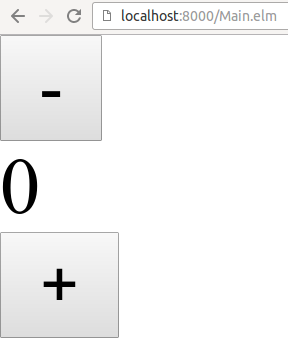
\includegraphics[scale=0.5]{img/counter.png}
	\caption{Ein simpler Zähler auf einer Webseite}\label{fig:counter}
\end{figure}
Die Abbildung~\ref{fig:counter} zeigt einen simplen Zähler der über zwei Knöpfe inkrementiert und dekrementiert werden kann. Der aktuelle Stand des Zählers wird zwischen den Knöpfen angezeigt und kann sowohl negative, als auch positive Werte annehmen.
Der angezeigte Zählerwert ist das sogenannte $Model$ und zeigt den aktuellen Status der Applikation an. Interagiert ein Nutzer nun mit einem der beiden Knöpfe um den Zähler zu erhöhen oder zu reduzieren, wird diese Aktion an die sogenannte $Update$-Funktion weitergegeben. Zusätzlich zur auszuführenden $Aktion$, bekommt diese Funktion auch noch das aktuelle $Model$, sprich den momentanen Zählerwert übergeben.
Die $Update$-Funktion nimmt sämtliche Einwirkungen durch den Nutzer von außen entgegen und wendet diese Aktionen auf das aktuelle $Model$ an. Das bedeutet in diesem konkreten Fall, dass das $Model$ erhöht oder reduziert wird. Dabei wird jedoch nicht das $Model$ direkt verändert, sondern ein neues $Model$ mit den geänderten Werten wird zurückgegeben, da sonst ein Seiteneffekt die Folge wäre. Damit dieser Vorgang zügig vonstatten geht, nutzt Elm persistente Datenstrukturen, womit nur die tatsächlich geänderten Attribute eines Models im neuen $Model$ gesetzt werden, die unveränderten Attribute hingegen werden übernommen.
Das Ergebnis der Update-Funktion wird weitergereicht an die $View$-Funktion. Sie beschreibt das Aussehen der Website, soll heißen wie das $Model$ dargestellt wird. Elm nutzt ein virtuelles \ac{DOM}, wodurch nur tatsächliche Änderungen im Browser angezeigt werden, anstatt dauerhaft das komplette \ac{DOM} stetig zu aktualisieren. Das \ac{DOM} beschreibt die Schnittstelle zum Datenzugriff auf das Objektmodell eines \ac{HTML}-Dokumentes.
Der Datenfluss in Elm wird noch einmal in Abbildung~\ref{fig:elm-model-view-update-concept} visualisiert.
\begin{figure}[h]
  \centering  
  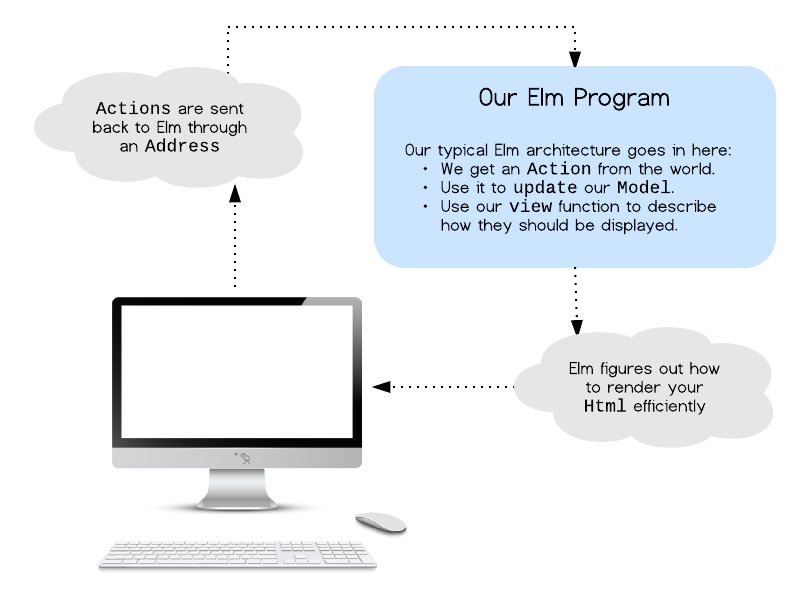
\includegraphics[scale=1]{img/elm-model-view-update-concept.png}
  \caption{Das Model-View-Update Konzept von Elm}\label{fig:elm-model-view-update-concept}
\end{figure}

\subsection{Umsetzung}
\label{sec:Umsetzung}
Der vom Programmierer verfasste Programmcode wird vor der endgültigen Nutzung zu \ac{JS}, \ac{HTML} und \ac{CSS} kompiliert und in die Webseiten integriert. Entsprechend fungiert in Elm verfasster Code im Endeffekt wie natives \ac{JS}, nutzt allerdings noch einige weitere vertiefende Konzepte, um viele Problematiken von \ac{JS} zu umgehen und auszumerzen.
Unter anderem verspricht Elm, dass generierter Code keinerlei Laufzeitfehler (http://elm-lang.org/) erzeugt. Sämtliche Fehlerquellen werden vom Compiler zuvor erkannt, abgefangen und an den Programmierer weitergeleitet, um sie zu beheben. Damit dies funktioniert, implementiert Elm mehrere Konzepte des deklarativen Programmierparadigmas.

\subsubsection{Keine Seiteneffekte}
\label{sec:Keine Seiteneffekte}
Ein Seiteneffekt beschreibt die mehrmalige Zuweisung einer Variable mit einem Wert. In Elm ist das allerdings nicht möglich. Sämtliche Variablen sind unveränderlich und können nur einmalig mit einem Wert initiiert werden. Danach bleibt diese Variable bis zum Ende der Laufzeit unverändert. Wie bereits beschrieben gibt es in Elm das Model, welches die Informationen über den Status der Applikation darstellt. Beschreibt das $Model$ beispielsweise den aktuellen Stand eines Zählers und wird dieser erhöht, muss auch das Model, um aktuell zu bleiben, verändert werden. Hier käme es zu einem Seiteneffekt. Realisiert wird diese Veränderung dadurch, dass ein neues Model mit den gleichbleibenden Daten, sowie dem zu ändernden, aktualisierten Wert erstellt wird. Da ein neues Model erstellt wurde, gibt es nun keinen Seiteneffekt mehr. Das vorherige $Model$ wird schlichtweg verworfen und mit einem neuen Model ersetzt.
Das Konzept der unveränderbaren Werte wurde aus der Mathematik übernommen.  Um Funktionen und ihre Korrektheit garantieren zu können, wird dort dasselbe Prinzip der unveränderlichen Variablen angewandt. Betrachtet man beispielsweise den Ausdruck~\ref{eq:imperative_equation}, so fällt auf, dass die Schreibweise lediglich in den meisten imperativen Programmiersprachen sinnvoll ist, allerdings einen Seiteneffekt darstellt.
\begin{equation} \label{eq:imperative_equation}
x = x + 1
\end{equation}
In einer imperativen Programmiersprache wird der Ausdruck~\ref{eq:imperative_equation} den aktuellen Wert in $x$ auslesen, um $1$ inkrementieren und das Ergebnis der Operation in die Variable $x$ schreiben.
Mathematisch betrachtet ist diese Aussage jedoch schlichtweg falsch, denn es existiert kein $x$, welches diese Aussage wahr werden lässt:
\begin{equation} \label{eq:mathematical_equation}
x=x+1 \leftrightarrow 0=1
\end{equation}
Die meisten imperativen Programmiersprachen nutzen das rechtsassoziative Gleichheitszeichen als Zuweisung, während es in der Mathematik als Vergleichsoperator angesehen wird.
Die eigentliche Bedeutung des Ausdrucks~\ref{eq:imperative_equation} ist mathematisch ausgedrückt:
\begin{equation} \label{eq:true_equation}
x_1:= x_0 + 1
\end{equation}
Es ist klar erkennbar, dass $x_1$ und $x_0$ nicht dieselbe Variable sind wodurch die Aussage nun als wahr eingestuft werden kann. Das beschriebene Konzept wird referentielle Transparenz genannt und beschreibt die Kontinuität des Wertes einer Variable.
Des Weiteren basieren Funktionen in Elm auf dem Konzept von reinen Funktionen($pure\,functions$). Das bedeutet, dass eine Funktion stets das gleiche Ergebnisse liefert, insofern auch die Eingabeparameter gleich bleiben, unabhängig vom Zeitpunkt der Ausführung. Beispiele für eine reine Funktion sind $sin(x)$ oder $add(x, y)$. Sie berechnen immer dieselben Werte, völlig unabhängig davon, wie oft oder zu welchem Zeitpunkt sie ausgeführt werden. Ein beliebtes Gegenspiel ist die $random()$ Funktion, die einen (semi-)zufälligen Wert zurückliefert und somit als eine unreine Funktion gilt. Doch auch diese Funktion kann zu einer reinen Funktion gemacht werden, wenn man sie einen Wert abhängig von einem Übergabeparameter berechnen lässt wie beispielsweise $random(seed)$.

\subsubsection{Elm-Compiler}
\label{sec:Elm-Compiler}
Laufzeitfehler sollen mit Elm in Vergessenheit geraten. Dafür soll der integrierte Compiler sorgen. Die Fehlermeldungen des Compilers sind sehr strikt und deuten exakt auf die Programmzeile die für den jeweiligen Fehler verantwortlich ist. Bei der herkömmlichen Entwicklung eines Frontends mit \ac{JS} trifft man häufig auf den Wert $undefined$. Dieser Wert beschreibt, dass die dazugehörige Variable noch nicht initialisiert wurde und somit keine nutzbaren Daten enthält. Trifft man nun auf diesen Wert und versucht eine andere Funktion darauf auszuführen, so kann das geschriebene Programm entsprechend abstürzen. Der Elm Compiler überprüft den Programmcode nach exakt diesen Situation beziehungsweise analysiert, ob Variablen und Funktionen vorab initialisiert wurden, welche Parameter die einzelnen Funktionen erwarten und ob die Rückgabeparameter dem Typen entsprechen, den die anderen Funktionen erwarten. Befolgt man die Anweisungen des Compilers, soll das in einem stark strukturierten, lesbaren und funktionieren Code münden.
Dem Programmierer werden weniger Möglichkeiten gegeben, bestimmte Ziele zu erreichen, doch dadurch soll auf lange Sicht einheitlicher, lesbarer und besser zu wartender Code erzeugt werden. Passend dazu gibt es bereits viele Erweiterungen für gängige Editoren wie Sublime Text und Atom, welche beim Speichern des Projektes den Code entsprechend des Style Guides strukturieren und formatieren. So kann einerseits die Lesbarkeit des Codes vereinheitlicht, andererseits die Fehlerquellen in Form von Einrückungsfehlern oder vergessenen Kommas o.ä. verringert werden.

\subsubsection{Statische Typisierung}
\label{sec:Statische Typisierung}
Anders als bei nativem \ac{JS}, gibt es in Elm keine dynamische Typisierung. Das bedeutet, dass sowohl die Typen einer Variable, als auch die Rückgabewerte von Funktionen bereits bei der Kompilierung bekannt sein müssen. Natives \ac{JS} erlaubt es, dass die Typen von Variablen erst zur Laufzeit überprüft werden und sich zusätzlich in dieser Zeit ändern können. So ist der Quellcode in Abbildung~\ref{fig:dynamische-typisierung} konform in \ac{JS}.
\begin{figure}[ht]
\begin{lstlisting}[language=JavaScript]
var i = 1;
i = "Test";
\end{lstlisting}
\caption{Beispiel der dynamischen Typisierung}\label{fig:dynamische-typisierung}
\end{figure}
Der Typ der Variable $i$ wurde in der Abbildung~\ref{fig:dynamische-typisierung} während der Laufzeit von $number$ zu $string$ geändert. Da Elm stark typisiert ist, gibt es keine Möglichkeit, dass eine Funktion verschiedene Datentypen zurück gibt oder eine Variable mehrere Typen während der Laufzeit annimmt.

\subsubsection{Modularität}
\label{sec:Modularität}
Um geschriebenen Code auch in Zukunft wartbarer zu machen, ist Elm modular aufgebaut und leicht erweiterbar. Es ist denkbar einfach vorhandenen Code zu importieren. Die importierten Module verstehen sich als gekapselt, wodurch sie in keiner Weise mit dem bereits verfügbaren Code kollidieren können.


\subsubsection{Performanz}
\label{sec:Performanz}
\begin{figure}[hb]
  \centering  
  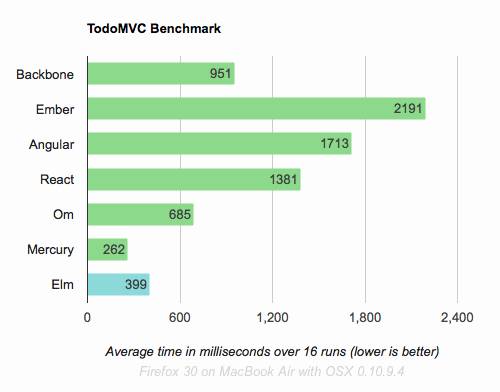
\includegraphics[scale=0.6]{img/virtual-dom.png}
  \caption{Performanz von Elm im Vergleich zu anderen Web-Frameworks. \cite{elm-performance}}\label{fig:performance}
\end{figure}
Obwohl Daten nicht verändert, sondern lediglich als neuer aktualisierter Datensatz betrachtet werden und einzelne Funktionen stark ausgelagert werden können, leidet die Performanz nicht darunter. Laut Abbildung~\ref{fig:performance} überzeugt Elm mit einer sehr guten Geschwindigkeit. Möglich wird das durch die Verwendung eines virtuellen \ac{DOM}.
Dabei wird das echte \ac{DOM} bei jedem „Frame“ in eine abstrakte Version kopiert. Auf diese abstrakte Version werden die Änderungen angewandt. Zunächst klingt diese Vorgehensweise sehr langsam und aufwändig, doch um die Geschwindigkeit zu gewährleisten wird das aktuelle abstrakte \ac{DOM} mit dem neuen, veränderten \ac{DOM} verglichen und nach Unterschieden gesucht. Jede Unterschiedlichkeit wird daraufhin zu einer Liste hinzugefügt, in der sämtliche Änderungen festgehalten werden. Anschließend wird diese Liste an den Browser zurückgegeben, so dass alle Änderungen für den Nutzer sichtbar gemacht werden können. Daraus resultiert, dass nur noch die tatsächlich neuen Elemente im \ac{DOM} des Nutzers aktualisiert werden müssen. Dieser zu verändernde Teil stellt nur einen Bruchteil des kompletten \ac{DOM} dar. Man kann dadurch von einer immensen Effizienzsteigerung ausgehen.


\subsubsection{Interoperabilität}
\label{sec:Interoperabilität}
Es wäre sehr aufwendig die gängigsten JavaScript-Bibliotheken und -Frameworks wie jQuery oder AngularJS komplett zu verwerfen und mit Elm zu realisieren respektive neu zu programmieren. Glücklicherweise bietet Elm eine ausgereifte Interoperabilität, wodurch alle Garantien der deklarativen Programmierung übernommen werden können, selbst wenn die externen Bibliotheken diese nicht gewährleisten.
Die genannten externen Bibliotheken sind zum Großteil nicht deklarativ programmiert, weswegen normalerweise keinerlei Garantien seitens Elm gemacht werden können. Jedoch ist Elm von den externen Bibliotheken isoliert und kommuniziert nur über sogenannte Ports mit JavaScript. Die Kommunikation durch die Ports funktioniert in beide Richtungen, womit sämtliche Daten bei Bedarf ausgetauscht werden können. Da in Elm wie bekannt vorab die Typen der Eingabeparameter und Rückgabewerte spezifiziert werden müssen, werden die Garantien weiterhin gewahrt.

\subsubsection{Debugger}
\label{sec:Debugger}
Nicht nur die detaillierten Fehlermeldungen des Compilers sind ein großer Pluspunkt von Elm, sondern auch der mitgelieferte und einfach zu bedienende Debugger. Anders als bei anderen Programmiersprachen zeigt der Debugger nicht nur einen einfachen Stacktrace mit den letzten Rücksprungadressen an. Vielmehr ermöglicht es der Debugger in Elm die Zeit zurückzudrehen. In gängigen Debuggern ist es nicht einfach, ein bestimmtes Verhalten, das möglicherweise zum Absturz des Programms geführt hat, zu reproduzieren. Um den Fehler erneut zu erhalten und dadurch ein Verständnis des Fehlers aufzubauen ist es oft notwendig den genauen Hergang und Ablauf manuell nachzuahmen. Der Elm Debugger hingegen speichert den Status einer jeden Variable zu jedem Zeitpunkt und zeichnet außerdem die Wechsel auf. Aufgrund dessen ist es sehr einfach möglich mit Hilfe eines Sliders auf der Website die Zeit buchstäblich zurückzudrehen und den vorherigen Status wieder aufzurufen. Weiterhin besteht die Möglichkeit sämtliche Daten zu diesem Zeitpunkt zu betrachten und live zu verändern. Dadurch wird nicht nur der aktuell begutachtete Status verändert und der Effekt zeitgleich auf dem Bildschirm angezeigt, sondern auch alle folgenden Status mitsamt den Daten werden entsprechend aktualisiert. Evan Czaplicki hat dahingehend ein Video angefertigt, dass den Vorgang sehr detailliert beschreibt (LINK). Alternativ kann die Abbildung XY betrachtet werden, die einen Zeitstrahl mit Werten, sowie die Möglichkeiten die sich durch den Debugger ergeben, aufzeigt.


\subsubsection{Praktische Anwendungsgebiete}
\label{sec:Praktische Anwendungsgebiete}
Elm ist noch recht neu und befindet sich im ständigen Wandel. Für viele Entwickler ist Elm entsprechend noch keine wirkliche Alternative zu ihren gegenwärtig genutzten Frameworks, obgleich die Entwicklung mit den gängigen Werkzeugen oftmals steinig ist. Nur wenige Unternehmen nutzen derzeit Elm in ihrem Produktionsumfeld. Die wohl derzeit größten Nutzer sind NoRedInk, Prezi und CircuitHub. Alle Betriebe überführen Stück für Stück bereits bestehende Teile ihres Frontends zu Elm. NoRedInk gibt an, dass der überführte Elm-Code in den letzten acht Monaten keinerlei Laufzeitfehler erzeugt hat, anders als die vorherige Implementierung\\ (https://www.youtube.com/watch?v=zBHB9i8e3Kc). Dennoch wird es wohl noch eine Weile dauern, bis sich mehr Firmen der Vorstellung hingeben ihr lauffähiges System in die vielversprechende Programmiersprache Elm zu portieren, nicht zuletzt, weil sie sich noch in einem sehr frühen Stadium befindet und somit noch nicht völlig ausgereift ist.
Es existiert jedoch bereits eine Vielzahl an Projekten die mit Elm verwirklicht wurden. Dabei sind viele dieser Projekte kleinere Retro-Spiele, die über den Browser gespielt werden können \footnote{\cite[vgl.]{builtwithelm}}. Dazu gehört unter anderem Tetris, Pong und Space Invaders. Weiterhin bietet Elm sehr einfache Möglichkeiten Formen wie Kreise, Vierecke, Hexagone und vieles mehr zu erzeugen, ohne großartig in die Mathematik einzusteigen.\\
Dieser Einblick zeigt bereits, dass Elm in vielerlei Hinsicht Besserung für die Entwicklung von Webapplikationen verspricht. Doch wie praktikabel sind diese Versprechungen? Ist die Programmiersprache effizient und intuitiv, oder durch ihr noch frühes Entwicklungsstadium unausgereift?
„The best functional programming in your browser“ - Diese Aussage wird anhand verschiedener Bewertungskriterien überprüft.
Im Zuge dessen wird eine Webseite mit kleineren Modulen in Elm erzeugt. Die fertige Webseite respektive der erzeugte Quellcode wird anhand der zuvor erstellten Bewertungskriterien ausgewertet. Auch die Beobachtungen während der Entwicklung, wie etwa unvorhergesehene Probleme, gehen mit in die Wertung ein.

\subsection{Einführung in die Elm-Architektur}
\label{sec:elm-architektur}
TODO: Evtl. Absatz \nameref{sec:Praktische Anwendungsgebiete} hier rein mergen und abändern?
... Um eine Programmiersprache jedoch anzuwenden, ist es notwendig zuvor die Architektur kennenzulernen. Dieses Kapitel soll eine Einführung in die Programmiersprache Elm darstellen und die grundlegenden Funktionen näher bringen.

\subsubsection{Elm-REPL}
\label{sec:elm-repl}
Ein nützliches Tool um mit Werten in Elm zu interagieren und kleinere Algorithmen zu testen, ist die $elm-repl$. \ac{REPL} bezeichnet dabei die Iteration, welche ein Algorithmus durchlebt. Zunächst wird der Quellcode gelesen (read), danach ausgewertet (evaluate) und das Ergebnis ausgegeben (print). Dieser Vorgang wiederholt sich (loop), bis die Entwicklung fertig ist. $Elm-repl$ wird über die Kommandozeile aufgerufen und gestartet. In Abbildung~\ref{fig:elm-repl} ist das Tool abgebildet und zeigt beispielhafte Eingaben und Evaluierungen.
\begin{figure}[h]
\centering
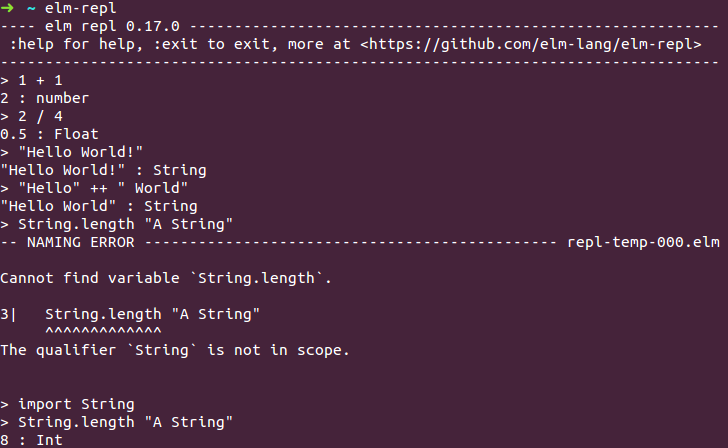
\includegraphics[scale=0.5]{img/elm-repl.png}
\caption{Das Tool elm-repl in der Kommandozeile}\label{fig:elm-repl}
\end{figure}
Wie aus der Abbildung~\ref{fig:elm-repl} ersichtlich wird, werden auch Fehler ausgegeben. In diesem Beispiel wurde versucht auf die Bibliothek $String$, genauer die Funktion $length$ zuzugreifen. Diese Bibliothek wurde allerdings noch nicht eingebunden, wodurch es zu dem Fehler kam. Nachdem die Bibliothek über das Kommando $import String$ importiert wurde, war der Fehler behoben. Die $elm-repl$ erlaubt es, alle Bibliotheken die das Paket $core$ mitliefert, zu importieren.

\subsubsection{Basisdatentypen}
\label{sec:Basisdatentypen}
Elm hat nur eine geringe Anzahl an Basisdatentypen, mithilfe derer sämtliche weiterführende Konstrukte abgeleitet werden können:
\begin{itemize}
	\item 42 : number
	\item True : Bool
	\item 'a' : Char
	\item {[1, 2, 3] : List}
\end{itemize}
Durch die Kombination dieser Basisdatentypen können weitere komplexere Datentypen wie $Strings$, $Integer$ oder $Floats$, wie es in Abbildung~\ref{fig:elm-repl} zu sehen ist, erzeugt werden.

\subsubsection{Basisfunktionen}
\label{sec:Basisfunktionen}
Elm kommt mit einer Vielzahl an grundlegenden Funktionen, um notwendige arithmetische Operationen zu ermöglichen. Dazu gehören Funktionen zur Addition ($+$), Subtraktion ($-$), Multiplikation ($*$) und Division ($/$). Um Vergleiche zu vollziehen gibt es die Funktionen zur Prüfung der Gleichheit ($==$) und Ungleichheit($/=$). Wie in Abbildung~\ref{fig:elm-repl} zu sehen ist, können zwei $String$s zu einem verbunden werden, indem die Funktion $++$ angewendet wird.

\subsubsection{Union Types}
\label{sec:Union-Types}
In vielen Applikationen können Datentypen unterschiedliche Zustände annehmen. So kann beispielsweise ein $Tag$ die Zustände $Montag$ bis $Sonntag$ annehmen. Die in anderen Programmiersprachen als $algebraische Datentyp$ bekannte Aufzählung von Zuständen wird in Elm $Union\,Type$ genannt und beschreibt auch hier eine Aufzählung von endlich vielen Zuständen eines Datentypen. Die Einführung eines solchen $Union\,Type$s erlaubt es dem Compiler den Quellcode auf fehlende Zustände zu überprüfen. Ist es zum Beispiel das Ziel, eine Meldung abhängig vom aktuellen Wochentag auszugeben, müssen alle Zustände und ihre Folge dafür deklariert werden. Fehlt eine Deklaration, kann der $Elm-Compiler$ dies anhand des $Union\,Type$s erkennen.
\begin{figure}[h]
\begin{lstlisting}[language=Elm]
type Day = Monday | Tuesday | .. | Sunday
storeStatus : Day -> String
storeStatus day =
  case day of
    Monday ->
      "Opened"
    Sunday ->
      "Closed"
\end{lstlisting}
\caption{Ein Union-Type in Elm}\label{fig:elm-union-type}
\end{figure}
Betrachtet man die Abbildung~\ref{fig:elm-union-type} ist klar erkennbar, dass die Funktion $storeStatus$ nicht alle Fälle, die der Typ $Day$ annehmen kann, behandelt werden. Aufgrund der vorherigen Deklaration eines $Union\,Type$ kann der $Elm-Compiler$ einsehen, welche möglichen Zustände der Typ $Day$ annehmen kann. Dadurch wird ein Fehler geworfen, insofern die fehlenden Typen nicht ergänzt werden. Dieses Konzept der algebraischen Datentypen erscheint zunächst sehr ähnlich den $Enumerationen$ in beispielsweise $C++$ oder anderen Programmiersprachen. Tatsächlich gibt es diese Form der Datenabstraktion in einer Vielzahl von funktionalen Programmiersprachen, mit dem wohl bekanntesten Vertreter der funktionalen Programmiersprache $Haskell$. Der Vorteil eines $Union\,Type$s in Elm gegenüber $Enumerationen$ in C++ oder Java ist, dass jeder Zustand der Aufzählung optionale Parameter übergeben bekommen kann. Damit bietet sich die Möglichkeit viel detailliertere Konstrukte zu erzeugen, ohne die Typensicherheit die sich durch die $Union\,Type$s ergibt zu verlieren. Das Beispiel der Abbildung~\ref{fig:elm-union-type} könnte entsprechend erweitert werden, so dass die Tage $Montag$ bis $Freitag$ zusätzlich noch eine Öffnungszeit besitzen.
\begin{figure}[h]
\begin{lstlisting}[language=Elm]
type Day = Monday Int Int | .. | Sunday
storeStatus : Day -> String
storeStatus day =
  case day of
    Monday start end->
      "Opened from:"
      	++ start "until"
      	++ end
    Sunday ->
      "Closed"
\end{lstlisting}
\caption{Ein erweiterter Union-Type in Elm}\label{fig:elm-union-type-advanced}
\end{figure}
Wie in Abbildung~\ref{fig:elm-union-type-advanced} zu sehen ist, wurden die einzelnen Tage in der Deklaration um die Parameter $Int$ erweitert. In diesem Fall sollen die $Integer$ vereinfacht die Start- und Endzeit der Öffnungszeit widerspiegeln. Auffällig ist, dass die Signatur der Funktion $storeStatus$ im Vergleich zur vorherigen Abbildung~\ref{fig:elm-union-type} nicht verändert wurde. Der übergebene Datentyp ist noch immer ein $Day$, mit dem Zusatz, dass die Wochentage zwei weitere Parameter $start$ und $end$ besitzen. Auf diese Weise können komplexe Konstrukte definiert werden, während die Typensicherheit gewährt bleibt.

\subsubsection{Records}
\label{sec:Records}
Eine weitere Datenstruktur in Elm sind die sogenannten $Records$. Ein $Record$ ist vergleichbar mit einem $Objekt$ in \ac{JS} und verfolgt eine sehr ähnliche Syntax. Es ist möglich, eigene Felder in einem $Record$ zu definieren, mit allen Datentypen die bisher erzeugt wurden. Dazu gehören nicht nur die Basis-Datentypen, sondern auch alle daraus konstruierten. Auch können verschiedene Datentypen in einem $Record$ kombiniert werden.
\begin{figure}[h]
\begin{lstlisting}[language=Elm]
university = { typ = "Fachhochschule"
             , gruendungsdatum = 1969
             , ort = "Kiel" }
university.typ  --> "Fachhochschule"
.ort university --> "Kiel"

{university | ort = "Flensburg" }
\end{lstlisting}
\caption{Ein Record in Elm}\label{fig:elm-record}
\end{figure}
In Zeile $1$ der Abbildung~\ref{fig:elm-record} ist erkennbar, wie ein $Record$ mit initialen Werten erstellt wird. Lediglich das Gleichheitszeichen für die Zuweisung unterscheidet sich hierbei von herkömmlichen erstellen eines $Records$ in \ac{JS}. Um ein Feld in einem $Record$ direkt anzusprechen, kann die übliche Schreibweise aus Zeile $4$ gewählt werden. Zeile $5$ hingegen führt zum gleichen Ergebnis, nutzt intern jedoch eine $anonyme\,Funktion$. Der Unterschied eines $Records$ im Gegensatz zu einem $Objekt$ in \ac{JS} liegt darin, dass Felder nicht dynamisch hinzugefügt oder gelöscht werden können. Sobald ein Feld definiert wurde, ist es für die gesamte Laufzeit vorhanden. Die einzige Möglichkeit einen $Record$ zu verändern liegt darin, den Inhalt der Felder zu manipulieren. Zeile $7$ der Abbildung~\ref{fig:elm-record} zeigt, wie das Feld $Ort$ des $Records$ mit einem neuen Wert versehen wird. Dabei ist zu beachten, dass aufgrund der Unveränderlichkeit einer Datenstruktur in Elm nicht der $Record$ selbst verändert wird. Viel mehr wird ein neuer $Record$ erstellt, der die Änderung, sowie gleichbleibenden Felder des alten $Record$ annimmt. Ein weiterer Unterschied gegenüber \ac{JS} ist, dass ein Feld nie den Wert $undefined$ oder $null$ annehmen kann, da eingeführte Felder stets initialisiert werden müssen. Des Weiteren ist es nicht möglich rekursive Felder zu erzeugen.

\subsubsection{Tupel}
\label{sec:Tupel}
Sollte es notwendig sein, mehr als einen Wert als Rückgabewert zu haben, so bietet sich die Nutzung von $Tupel$n an. Ein $Tupel$ ist eine weitere Datenstruktur in Elm und kann eine beliebig feste Anzahl an Werten beinhalten. Jeder Wert ist unabhängig von den anderen und kann einen geeigneten Datentyp annehmen. Die folgende Abbildung~\ref{fig:elm-tupel} zeigt, wie ein solches Tupel von einer Funktion zurückgegeben werden kann.
\begin{figure}[h]
\begin{lstlisting}[language=Elm]
type Food = { name: String, sort: String }

isCookie : Food -> (Bool, String)
isCookie food =
  if food.sort == "cookie" then
    (True, food.name)
  else
    (False, "No cookie.")

isCookie { name = "Oreo", sort = "cookie" }
--> (True, "Oreo")
\end{lstlisting}
\caption{Ein Tupel in Elm}\label{fig:elm-tupel}
\end{figure}
Der Rückgabewert des beispielhaften Aufrufes in Zeile $10$ ist ein Tupel, bestehend aus einem $Bool$ und einem $String$, wie es in der Signatur in Zeile $3$ definiert wurde. Soll das Tupel noch weiter verwendet werden, liefert die Bibliothek $Basics$ aus dem Paket $elm-lang/core$ die Funktionen $fst$ und $snd$, die entsprechend den ersten oder zweiten Wert eines Tupels zurückliefern. Auf diese Weise kann ein einzelner Wert des Tupels extrahiert werden. Aufgrund der fehlenden Wege Tupel mit mehr als zwei Werten auszuwerten, sollte nur bedingt auf Tupel zurückgegriffen und stattdessen ein $Record$ verwendet werden.

\subsubsection{Variablen}
\label{sec:Variablen}
Die Lebenszeit eines $Records$ ist die gesamte Laufzeit des Programmes. Eine $Variable$ in Elm hingegen bleibt nur für die Dauer der Funktion in der sie definiert wurde erhalten und ist auch nur in diesem Namensraum gültig. Außerhalb der Funktion ist die Variable nicht mehr bekannt. In Elm wird eine Variable innerhalb eines $let..in$-Konstrukts erzeugt. $Let$ bezeichnet dabei den Abschnitt, in welchem sämtliche Variablen erstellt werden und einen Wert zugewiesen bekommen. Die innerhalb dieses Blockes definierten Variablen können dabei aufeinander zugreifen, unabhängig von ihrer Reihenfolge. Mit Hilfe des $let..in$-Blockes kann die Logik einer Funktion noch weiter ausgelagert werden, ohne eine explizit neue Funktion zu definieren.
\begin{figure}[h]
\begin{lstlisting}[language=Elm]
meaningOfLife =
  let
    fourtyTwo = oneHundred - 58
    oneHundred = 100
  in
    fourtyTwo

meaningOfLife --> 42
\end{lstlisting}
\caption{Eine Variablendeklaration in Elm}\label{fig:elm-variables}
\end{figure}
Abbildung~\ref{fig:elm-variables} zeigt beispielhaft die Deklaration einer Funktion $meaningOfLife$, die innerhalb des $let..in$-Blockes die Variablen $fourtyTwo$ und $oneHundred$ deklariert und ihnen einen Wert zuweist. Die Inhalte eines $let..in$-Blockes müssen eingerückt werden, während hingegen eine übliche Funktion auch in einer Zeile verfasst werden kann. Des Weiteren ist erkennbar, dass die Variable $oneHundred$ erst nach der Deklaration von $fourtyTwo$ deklariert wird, jedoch bereits vorher nutzbar ist. Der $elm-compiler$ optimiert diese Programmstelle während des Kompiliervorganges entsprechend. Die beiden deklarierten Variablen sind lediglich in dem definierten $let..in$-Block verfügbar. Eine Verwendung außerhalb des Blockes hätte einen Compilerfehler zur Folge. Es besteht ferne die Möglichkeit ganze Funktionen innerhalb des Blockes zu definieren und zu nutzen.

\subsubsection{Kontrollstrukturen}
\label{sec:Kontrollstrukturen}
Elm bietet die Möglichkeit verschiedene Kontrollstrukturen anzuwenden. Dabei wird ein Record auf mögliche Werte hin überprüft und abhängig vom Wert ein anderer logischer Pfad gewählt.
\begin{figure}[h]
\begin{lstlisting}[language=Elm]
isItACookie food =
  if food == "cookie" then
  	True
  else if food == "grapefruit" then
    False
  else
    False
\end{lstlisting}
\caption{Eine Konstrollstruktur in Elm}\label{fig:elm-conditional}
\end{figure}
In Abbildung~\ref{fig:elm-conditional} ist eine herkömmliche $if$-Abfrage zu sehen. In Elm sind die Schlüsselwörter $if$, $then$ und $else$ notwendig und unterteilen die Bedingung von der angewandten Folge, die nach dem Schlüsselwort $then$ folgt. Insofern keine $if$-Bedingung zutrifft, wird der $else$-Fall angewandt.
Elm verfolgt auch hier die statische Typisierung und fordert, dass jede mögliche Verzweigung denselben Typen zurückliefert. Eine Bedingung muss in Elm immer $True$ oder $False$ liefern und somit einen $Bool$ liefern. In anderen Programmiersprachen wie beispielsweise $C++$ evaluiert eine Bedingung zu $True$, wenn sie nicht $0$ oder $false$ ist. Am Beispiel in Abbildung~\ref{fig:cpp-conditional} sieht man, dass $0$ zu $false$ auswertet. In Elm hingegen meldet der $elm-compiler$ einen Fehler, sobald eine Bedingung zu einem anderen Typen als $Bool$ auswertet.
Abbildung~\ref{fig:elm-union-type} zeigt, wie $Union\,Type$s überprüft werden können. Die Kontrollstruktur ähnelt dabei dem $switch$-$case$-Konstrukt von anderen Programmiersprachen wie \ac{JS} oder C++.
\begin{figure}[h]
\begin{lstlisting}[language=cpp]
string whatIsZero() {
  if (0) return "0 equals to TRUE";
  else return "0 equals to FALSE";
}
cout << whatIsZero() << endl;
//=> 0 equals to FALSE

\end{lstlisting}
\caption{Konstrollstruktur in C++}\label{fig:cpp-conditional}
\end{figure}

\subsubsection{Funktionen}
\label{sec:Funktionen}
Um in irgendeiner Art und Weise eine Interaktion mit den erstellten $Records$ zu vollziehen, benötigt der Entwickler auch in Elm eine Funktionen. Solch ein Programmkonstrukt wird mittels eines Funktionsnamen und dem Gleichheitszeichen realisiert.
\begin{figure}[h]
\begin{lstlisting}[language=Elm]
add : Int -> Int -> Int
add a b =
  a + b

add 3 4  --> 7
\end{lstlisting}
\caption{Eine Funktion in Elm}\label{fig:elm-function}
\end{figure}
Abbildung~\ref{fig:elm-function} zeigt, wie eine simple Addition zweier Integer-Werte umgesetzt wird. Die Buchstaben $a$ und $b$ deuten an, dass die Funktion $add$ zwei Parameter erwartet. Der gesamte Inhalt nach dem Gleichheitszeichen ist der sogenannte Rumpf einer Funktion und beschreibt den anzuwendenden Algorithmus. Der Funktionsaufruf ist in Zeile 5 sichtbar. Auffällig ist, dass eine Funktion nie explizit einen Wert zurück gibt, wie es in anderen Programmiersprachen wie \ac{JS} oder C++ meist durch den Befehl $return$ geschieht. Elm gibt implizit die letzte ausführbare Zeile als Rückgabewert zurück. Der beispielhafte Aufruf der Funktion $add$ in Zeile 5 hätte dementsprechend $7$ als Ergebnis. Des Weiteren ist erkennbar, dass Elm ohne die Nutzung von Kommata oder Klammern auskommt. Klammern werden erst notwendig, wenn mehrere Funktionen geschachtelt ablaufen sollen und eine Auswertung der Befehle von links nach rechts nicht ausreicht.
Zusätzlich zu einer explizit benannten Funktion, gibt es die $anonyme$ Funktion. Sie kommt ohne einen Funktionstitel aus und wird an Funktionen höherer Ordnung weitergereicht.
$List.filter$ ist eine solche Funktion und erwartet eine anonyme Funktion als Parameter, auf Basis derer eine Liste gefiltert wird. Aus der Abbildung~\ref{fig:elm-anonym-function} wird ersichtlich, dass die übergebene Liste, bestehend aus $4$ Einträgen, auf die Präsenz des Buchstabens $a$ hin überprüft wird. Dabei wird jeweils ein Wert an die anonyme Funktion weitergereicht, die in Form der Variable $str$ repräsentiert und mit dem String $a$ auf Gleichheit überprüft wird. Einträge die diesem Vergleich entsprechen, werden einer neuen Liste hinzugefügt. Wird das Ende der zu überprüfenden Liste erreicht, wird die Ergebnisliste als Rückgabewert ausgegeben.

\subsubsection{Signaturen}
\label{sec:Signaturen}
Die jeweils erste Zeile der Abbildung~\ref{fig:elm-function} und \ref{fig:elm-anonym-function} zeigt den Aufbau einer Signatur. Solch eine Signatur beschreibt die Funktion. Dabei sind Informationen über die Anzahl und der jeweilige Typ der Übergabeparameter, sowie der Typ des Rückgabewertes enthalten. Der letzte Typ einer Signatur ist dabei immer der Rückgabewert, die vorherigen Typen stellen die Typen der Übergabeparameter in der übergebenen Reihenfolge dar. Die einzelnen Parameter sind durch einen Pfeil ($->$) voneinander getrennt. Wird eine Funktion anstelle eines einfachen Datentypen als Parameter übergeben, wird dies wie in Abbildung~\ref{fig:elm-anonym-function} durch das Einklammern der Typen angedeutet. Die Typen innerhalb der Klammer stellen wiederum die Typen der Übergabeparameter und Rückgabewerte der Funktion dar.
\begin{figure}[h]
\begin{lstlisting}[language=Elm]
List.filter : (a -> Bool) -> List a -> List a
List.filter (\str -> str == "a") ["a", "b", "c", "a"]
--> ["a", "a"]
\end{lstlisting}
\caption{Anwendung einer anonymen Funktion in Elm}\label{fig:elm-anonym-function}
\end{figure}
Anhand der Abbildung~\ref{fig:elm-function} lässt sich erkennen, dass die $add$-Funktion zwei Parameter vom Typ $Int$ erwartet und letzten Endes ein Ergebnis des Typ $Int$ liefert. Fehlt einer Funktion die Signatur, wird der $elm-compiler$ eine Warnung ausgeben und zusätzlich eine passende, jedoch teilweise allgemeinere Signatur ausgeben. Würde die Funktion in Abbildung~\ref{fig:elm-function} keine Signatur enthalten, würde der $elm-compiler$ die Signatur $add : number -> number -> number$ vorschlagen. Da ein $Int$ nur eine Spezifizierung des Basisdatentypen $number$ darstellt, ist das nicht verwunderlich. Der $elm-compiler$ nutzt implizit die eigens erarbeiteten Signaturen bei der Überprüfung des Quellcodes, sollte der Entwickler keine Signatur angegebenen haben.

\subsubsection{Typen Alias}
\label{sec:typ-alias}
Je komplexer ein Record wird, desto länger und unübersichtlicher wird auch die dazugehörige $Signatur$. Dementsprechend bietet sich eine Abkürzung der Signatur an, die in Elm als $type\,alias$ bezeichnet wird. Dabei handelt es sich um eine Repräsentation einer komplexen Datenstruktur in einer kurzen Schreibweise.
\begin{figure}[h]
\begin{lstlisting}[language=Elm]
isOldEnough : { name : String
	      , profile : String
	      , age : Int
	      } -> Bool
isOldEnough user =
	...
\end{lstlisting}
\caption{Definition einer Funktion ohne Typen Alias}\label{fig:no-type-alias}
\end{figure}
In Abbildung~\ref{fig:no-type-alias} wird eine Funktion mit einem komplexen $Record$ als Übergabeparameter beschrieben. An dieser Stelle hat der $Record$ lediglich drei Felder, führt allerdings schon zu einem recht unübersichtlichen Quellcode. Mit Hilfe des $type\,alias$ kann die Signatur gekürzt werden, indem die Repräsentation des $Records$ ausgelagert wird. In Abbildung~\ref{fig:no-type-alias} können die Auswirkung davon betrachtet werden. Nachdem der $type\,alias$ erstellt wurde, kann das Konstrukt mit dem entsprechenden $alias$ angesprochen werden. Zeile $5$ verdeutlicht, wie der $alias$ genutzt wird. Der Algorithmus der Funktion bleibt völlig unberührt, wodurch diese Änderung eher kosmetischer Natur ist.
\begin{figure}[h]
\begin{lstlisting}[language=Elm]
type alias User = { name : String
	          , profile : String
	          , age : Int
	          }
oldEnough : User -> Bool
\end{lstlisting}
\caption{Definition einer Funktion mit Typen Alias}\label{fig:type-alias}
\end{figure}

\subsubsection{Module}
\label{sec:Module}
\begin{figure}[h]
\begin{lstlisting}[language=Elm]
module MyModule exposing(..)
module MyModule exposing (add, anotherMethod)
\end{lstlisting}
\caption{Mögliche Deklarationen eines Elm-Moduls}\label{fig:elm-module}
\end{figure}
Oftmals ist es sinnvoll Quellcode der sich nur auf eine Problemlösung bezieht zu gruppieren. Auch in Elm ist es möglich Code auszulagern in sogenannte $Module$. Sie beschreiben eine Art Container, in dem der Code isoliert von den anderen Projektteilen betrachtet werden kann. Um ein $Modul$ in Elm zu erstellen, muss eine neue Datei vom Typ $elm$ erzeugt werden. Abbildung~\ref{fig:elm-module} zeigt zwei Beispiele, wie eine Quelldatei als Modul deklariert werden kann. Zeile $1$ gibt dabei sämtliche Funktionen die im Modul beinhaltet sind nach außen weiter, sobald das Modul importiert wird. Dies sollte nur gemacht werden, wenn das Modul sich um eine Art Bibliothek handelt, in der sämtliche Funktionen verfügbar gemacht werden sollen. In Zeile $2$ hingegen wird ersichtlich, wie nur ausgewählte Funktionen nach außen sichtbar gemacht werden. Auf der anderen Seite hingegen würde der Entwickler das Modul $MyModule$ importieren und daraufhin die Funktionen $add$ und $anotherMethod$ nutzen können.

\subsubsection{Importierung}
\label{sec:Importierung}
Jeder Entwickler hat ferner die Möglichkeit die zuvor erstellten Module an einer anderen Stelle zu importieren. Dabei wird das gesamte Modul in den aktuellen Namensraum geladen und nutzbar gemacht. In welcher Ausprägung die Funktionen des importierten Moduls eingebunden werden, hängt von der Spezifikation des Imports ab.
\begin{figure}[h]
\begin{lstlisting}[language=Elm]
import MyModule
import MyModule exposing(..)
import MyModule exposing (add, anotherMethod)
import MyModule as MyVeryOwnModuleName
\end{lstlisting}
\caption{Mögliche Formen der Importierung eines Elm-Moduls}\label{fig:elm-import-module}
\end{figure}
Die Abbildung~\ref{fig:elm-import-module} zeigt vier mögliche Arten das Modul $MyModule$ zu importieren. Zunächst einmal werden alle Funktionen, die das Modul selbst über das Stichwort $exposing$ freigibt geladen. Das Einbinden wie in Zeile $1$ hat zur Folge, dass sämtliche Funktionen mit dem expliziten Modulnamen voran angesprochen werden müssen. Die Funktion $add$ wird beispielsweise mit $MyModule.add$ aufgerufen. Zeile $2$ wiederum hat zur Folge, dass alle Funktionen des Moduls $MyModule$, darunter auch die Funktion $add$, in den Namensraum des aktuellen Moduls geladen werden. Logischerweise ist an dieser Stelle für den Aufruf der $add$-Funktion nichts weiter notwendig, außer wenn das aktuelle Modul eine gleichnamige Funktion besitzt. In diesem Fall ist die Nutzung analog der Anwendung aus dem vorherigen Beispiel. Die Einbindung in Zeile $3$ wirkt sich reduzierender auf den aktuellen Namensraum aus. Damit ist gemeint, dass nur die explizit genannten Funktionen nach dem Stichwort $exposing$ in den Namensraum geladen werden, alle anderen Funktionen müssen mit dem entsprechenden Modulnamen vorweg angesprochen werden. Schlussendlich kann der Namensraum des eingebundenen Moduls durch den Zusatz des $as$ Stichwortes, gefolgt vom gewünschten Namensraum verändert werden. Die Nutzung der Funktionen ist analog zu den vorherigen Beispielen und kann beliebig kombiniert werden.


\subsubsection{Online-IDE}
\label{sec:Online-IDE}
Damit begonnen werden kann mit Elm zu programmieren, ist es nicht notwendig sämtliche Tools auf dem lokalen Gerät zu installieren. Vielmehr haben die Entwickler von Elm eine Online-\ac{IDE} erstellt, mit der sofort online entwickelt werden kann.
\begin{figure}[h]
	\centering
	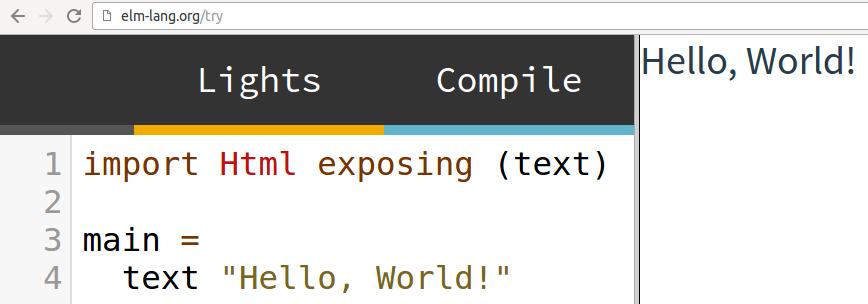
\includegraphics[scale=0.4]{img/elm-try.png}
	\caption{Die Online-\ac{IDE} von Elm}\label{fig:elm-try}
\end{figure}
Die Abbildung~\ref{fig:elm-try} zeigt diese \ac{IDE} mit einem typischen $Hello-World$ Beispiel. Auf der linken Seite ist eigentliche \ac{IDE} erkennbar, während die rechte Seite das Ergebnis nach dem Kompiliervorgang ausgibt. Sollte es einen Fehler während des kompilierens geben, wird die entsprechende Fehlermeldung des $elm-compiler$ dort ausgegeben. Mit Hilfe der Schaltfläche $Lights$ können zum Einen die Farben der \ac{IDE} invertiert werden, während der Knopf $Compile$ den geschriebenen Quellcode kompiliert und ausführt. Kleinere Projekte können entsprechend bequem mit diesem Tool realisiert werden. Die \ac{IDE} bietet einen schnellen Einstieg in die Programmiersprache.


\subsubsection{Installation}
\label{sec:Installation}
Die Online-\ac{IDE} bietet einen schnellen Einstieg in die Programmiersprache, ohne Programme lokal installieren zu müssen. Jedoch sind manche Konzepte nicht in der Online-\ac{IDE} nutzbar, so dass Elm lokal installiert werden muss. Das ist beispielsweise der Fall, sobald spezifische Pakete aus des Paketmanager von Elm installiert und benutzt werden möchten. Mehr Informationen über den Elm-eigenen Paketmanager folgen in der Sektion~\nameref{sec:start-eines-projektes}.

Die Elm-Webseite liefert Anleitungen um Elm auf Windows, Mac und allen NodeJs-kompatiblen Betriebssystemen zu installieren. Im folgenden werden die Kommandos zur Installation von Elm und dem \ac{NPM} unter Ubuntu 14.04 64bit erläutert, da der praktische Teil dieser wissenschaftlichen Arbeit unter diesem Zielsystem vorgenommen wurde.
Die Programmiersprache Elm wird über den \ac{NPM} verbreitet und muss somit zuvor installiert werden. Da der \ac{NPM} wiederum auf der Platform NodeJs basiert, muss auch das dazugehörige Paket installiert werden. Für die Installation sind die Kommandos aus Abbildung~\ref{fig:npm-install} in der Kommandozeile auszuführen.
\begin{figure}[h]
\begin{lstlisting}[language=bash]
$ sudo apt-get update
$ sudo apt-get install nodejs
$ sudo apt-get install npm
\end{lstlisting}
\caption{Installation des \ac{NPM}}\label{fig:npm-install}
\end{figure}
Dadurch wird das NodeJs-Paket installiert und ausführbar gemacht. Anschließend sollte überprüft werden, ob die Installation erfolgreich war und sowohl NodeJS, als auch der \ac{NPM} verfügbar sind.
\begin{figure}[h]
\begin{lstlisting}[language=bash]
$ node -v && npm -v
$ npm install -g elm
\end{lstlisting}
\caption{Installation von Elm}\label{fig:npm-install-check}
\end{figure}
Das Kommando in Zeile $1$ der Abbildung~\ref{fig:npm-install-check} liefert ein Ergebnis, wie es in Abbildung~\ref{fig:npm-installed} zu sehen ist. Elm kann nun über den \ac{NPM} mit dem Kommando aus Zeile $2$ installiert werden. Das Kürzel $-g$ installiert die neueste Elm-Version global für alle Projekte auf dem System. Entfernt man es, wird die Zielversion nur für den aktuellen Ordner zugänglich gemacht. Um die in dieser wissenschaftlichen Arbeit behandelte Version $0.17$ zu installieren, ist der Zusatz $@0.17$ direkt hinter dem globalen Flag notwendig. Nachdem alle Kommandos fehlerfrei ausgeführt wurden sollte Elm über die Konsole nutzbar sein.
\begin{figure}[hb]
\centering
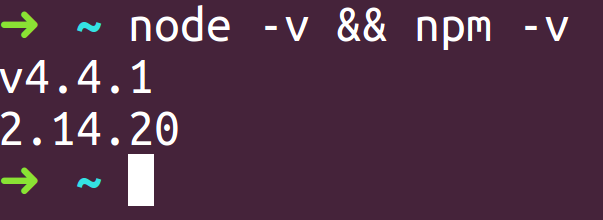
\includegraphics[scale=0.3]{img/npm-nodejs-installation.png}
\caption{Überprüfung der erfolgreichen Installation von NodeJs und dem \ac{NPM}}\label{fig:npm-installed}
\end{figure}


\subsubsection{Start eines Projektes}
\label{sec:start-eines-projektes}
Nachdem die Installation von Elm erfolgreich war, kann nun ein neues Projekt lokal erstellt werden. Dazu gehört zunächst einmal die Initialisierung des Projektordners, wodurch notwendige Ordner erstellt und Pakete installiert werden. Die Entwickler von Elm stellen dafür den Paketmanager $elm-package$ bereit. Dieses Tool wird zur Installation von externen Modulen, sogenannte Bibliotheken oder Pakete, benutzt. Zusätzlich hilft der Paketmanager dabei, das eigene Projekt lauffähig zu halten und nicht durch auftretende Aktualisierungen einzelner Pakete die Lauffähigkeit des eigenen Projektes zu verletzen. Dabei verfolgen die Entwickler des Paketmanagers bestimmte Versionsregeln, die auf jedwede Änderung an einem Paket angewendet wird. Alle Versionsnummern haben dabei genau drei Felder $MAJOR.MINOR.PATCH$, wobei der Beginn der Versionsnummern stets $1.0.0$ ist. Die Felder der Versionsnummern ändern sich abhängig der Änderungen an der API eines Paketes. Die harmloseste Änderung ist dabei der $PATCH$. Das bedeutet, dass die \ac{API} unverändert ist und keinerlei Gefahr für die Lauffähigkeit besteht. Es kann sich hierbei um beispielsweise Verbesserungen eines Algorithmus oder andere interne Änderungen handeln, die jedoch für den außenstehenden Entwickler keine Bedeutung haben.
Der nächstgrößere Schritt stellt die Aktualisierung der $MINOR$ Versionsnummer dar. Wie bei der Aktualisierung auf die nächste $PATCH$-Version, ist auch hier eine Aktualisierung unbedenklich. Das $MINOR$-Feld sagt aus, dass neue Methoden hinzugefügt wurden, alte Methoden jedoch unberührt blieben.
Wichtige Änderungen an einem Paket bei der alte Methoden maßgeblich verändert, oder sogar gelöscht wurden, werden mit dem Feld $MAJOR$ ausgedrückt. Hat sich dieses Feld verändert, wird eine Aktualisierung aller Wahrscheinlichkeit nach dazu führen, dass ein Programm nicht mehr lauffähig ist und Änderungen am eigenen Quellcode vorgenommen werden müssen.
Nutzt ein Entwickler beispielsweise das Paket $elm-lang/html\,1.2.3$, wird es voraussichtlich kompatibel mit allen zukünftigen Versionen bis Version $2.0.0$ sein. Ab diesem Zeitpunkt sind die vorgenommenen Änderungen so massiv, dass eine Aktualisierung nicht ohne weiteres möglich ist. Der Paketmanager $elm-package$ erzwingt die beschriebene Versionierung bei jedem Paket, bevor es veröffentlicht werden kann.TODO: \cite{https://github.com/elm-lang/elm-package}.
\begin{figure}[h]
\centering
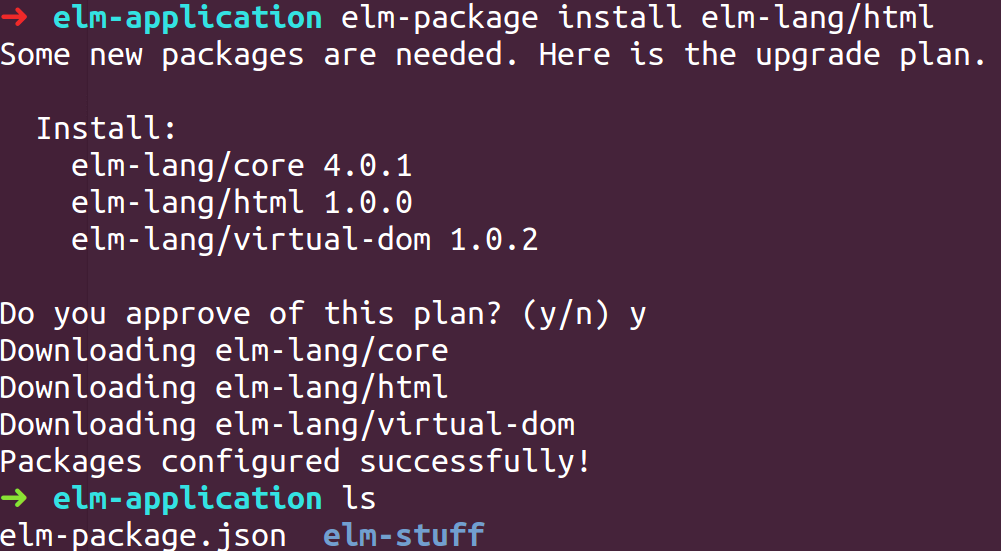
\includegraphics[scale=0.3]{img/elm-setup.png}
\caption{Installation eines externen Paketes über den Elm-Paketmanager}\label{fig:elm-install-package}
\end{figure}
Die Abbildung~\ref{fig:elm-install-package} zeigt, wie ein Paket installiert und der Projektordner eingerichtet wird. Der Paketmanager installiert nach der Bestätigung das angeforderte Paket und alle darin enthaltenen, externen Abhängigkeiten. Des Weiteren wird die Datei $elm-package.json$ erstellt, mit grundlegenden Informationen über das eigene Projekt, wie beispielsweise die Versionsnummer, eine Zusammenfassung oder die zu verwendende Lizenz, sowie eine Liste von installierten externen Paketen. Der Ordner $elm-stuff$ enthält die zuvor installierten Pakete. Nun muss noch manuell eine $.elm$-Datei erstellt werden, üblicherweise mit dem Namen des Projektes. In dieser Datei können die zuvor gezeigten Konzepte genutzt werden, um das gewünschte Programm zu verwirklichen.


\subsubsection{Fertigstellung}
\label{sec:elm-compile}
Zum Kompilieren eines Elm-Programmes wird das Tool $elm-make$ genutzt. Es kompiliert den gesamten Quellcode eines Ordners, oder die Dateien, welche dem Befehl hinzugefügt wurden. Ferner kann der Entwickler entscheiden, ob eine $.html$-Datei erstellt werden soll, in der bereits das kompilierte Elm-Programm eingebaut wird, oder eine $.js$-Datei, so dass das Einbinden oder die Auslieferung selbstständig vorgenommen werden kann.

\subsubsection{Elm Reactor}
\label{sec:elm-reactor}
\begin{figure}[h]
\centering
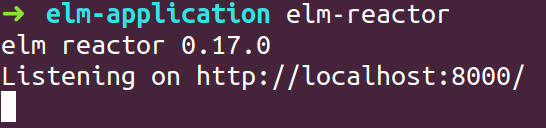
\includegraphics[scale=0.5]{img/elm-reactor.png}
\caption{Der gestartete Elm-Webserver}\label{fig:elm-reactor}
\end{figure}
Erklärung des Elm-Reactors. Siehe Evaluierung, der auskommentierte Teil.

\subsubsection{NULL/Undefined/Maybe in Elm?}
\label{sec:elm-undefined-null-maybe}
Konzept des Maybe erklären, da es auch in der Applikation mit den initialen Übergabeparametern genutzt wird.

\chapter{Evaluierung der Programmiersprache Elm}
\label{sec:Evaluierung der Programmiersprache Elm}
\pagestyle{plain}

\section{Bewertungsmuster}
\label{sec:Bewertungsmuster}
Der folgende Teil dieser wissenschaftlichen Arbeit befasst sich mit der Entwicklung eines Modells, um die Programmiersprache Elm und ihre Nutzung als Frontend für Webapplikationen bewerten zu können. Dabei soll ein bereits fertiges Template von den ursprünglichen Programmiersprachen HTML, CSS und JavaScript in die Programmiersprache Elm portiert werden. Während der Entwicklung/Portierung wird dann die Programmiersprache Elm gegenüber mehreren Gesichtspunkten verglichen und ausgewertet.
Das fertige Template ist eine Single-Page-Applikation mit Elementen, wie sie typischerweise auf einer solchen Webseite vertreten sind. Eine Single-Page-Applikation ist, wie der Name bereits suggeriert, eine Webseite effektiv nur einer aktiven Seite und ohne Unterseiten (ausgenommen Impressum, AGB und Datenschutz). Die SPA wird genutzt um ein Produkt oder Konzept schnell und einfach zu präsentieren, ohne den Nutzer mit Informationen zu überfluten und Unübersichtlichkeit in Form von tief verlinkten Unterseiten zu erzeugen. Oftmals wird eine SPA auch als Startseite benutzt und bietet nur eine geringe Anzahl an Funktionen.
Die fertige SPA soll unter anderem die folgenden, typischen Elemente enthalten:
\begin{itemize}
\item Navigation mit Anchor-Elementen
\subitem{-} Verkleinern der Navigation nach $x$ Pixeln
\subitem{-} ScrollSpy zur Darstellung der aktuellen Position
\item Titelbild mit einem vertikal und horizontal zentriertem Text
\item Service-Sektion
\item Twitter-Bootstrap CSS + Funktionen
\subitem{-} Vorgefertiges, responsive Design
\subitem{-} Hamburger Menü
\item Portfolio mit Bildern, wobei ein Klick einen asynchronen Request ausführt und Daten nach lädt
\item Formular zur Kontaktaufnahme mit Validierung der Korrektheit der eingegebenen Daten
\end{itemize}
Mit diesen Elementen kann eine typische SPA verwirklicht werden. Die Navigation bietet dabei die Möglichkeit für den Nutzer schnell zwischen einzelnen Sektionen der Seite zu wechseln. Das initiale Titelbild mit einem zentrierten Text gibt den Kontext der Präsentation an und soll das Interesse des Nutzers anregen. Die folgende Service-Sektion wird dazu genutzt, allgemeine Informationen über das beworbene Produkt anzuzeigen. In der darauf folgenden Portfolio-Sektion werden dem Nutzer mehrere Bilder des Produktes angezeigt, wobei ein Klick auf eines der Bilder dazu führt, dass ein Popup erzeugt wird in welches mit Hilfe eines AJAX-Requests Informationen asynchron vom Server angefordert und im Nachhinein geladen werden. Zuletzt kann sich der Nutzer für einen Newsletter anmelden. Die Eingaben des Nutzers sollen auf Richtigkeit überprüft werden.


\section{Bewertungskriterien}
\label{sec:Bewertungskriterien}
Während der Bearbeitung, respektive Überführung des Templates soll der erzeugte Code, sowie der Weg dahin analysiert werden. Hierbei sind Aspekte wie Wiederverwendbarkeit und Effizienz von großer Bedeutung. Aber auch die Produktivität während der Arbeit mit dem Code soll betrachtet werden. Die Bewertungskriterien setzen sich zum Großteil aus den zugrunde liegenden Kriterien aus dem Dokument XY der Washington University zusammen. Im Folgenden soll die Notwendigkeit der Kriterien und ihre eigentliche Bedeutung verständlich gemacht werden.
\iffalse
Dabei werden die Kriterien unterteilt in zwei Gruppen. Die erste Gruppe stellt externe Abhängigkeiten dar, also die Ansprüche eines Entwicklers an die Programmiersprache. Die zweite Gruppe zeigt interne Abhängigkeiten auf und setzt sich über die stark subjektiven Ansprüche und Einflüsse eines Entwicklers hinweg und versucht die Programmiersprache objektiv einzuordnen.

(http://www.cs.gordon.edu/courses/cs323/lectures-2009/LanguageEvaluationCriteria.pdf + http://courses.cs.washington.edu/courses/cse341/02sp/concepts/evaluating-languages.html)
\fi


\subsection{Entwicklungsgeschwindigkeit}
\label{sec:Entwicklungsgeschwindigkeit}
Gerade für Startups ist es wichtig, ein erstes Produkt so schnell wie möglich bereitzustellen. Die Entwickler müssen also mit wenigen Mitteln ein fertiges (Software-)Produkt ausliefern können, selbst wenn sie noch kein oder wenig Vorwissen zu einer Programmiersprache haben.
Dementsprechend sollte eine Programmiersprache nur eine geringe Anzahl an primitiven Konzepten aufweisen, die sich leicht erweitern lassen. Beispielsweise hat die Programmiersprache C standardmäßig keine Anreihung von Buchstaben, auch bekannt als $String$. Jedoch gibt es den Datentyp $char$, der einen einzelnen Buchstabe repräsentiert. Durch die Verknüpfung mehrerer $char$'s, kann letztendlich der Datentyp $String$ umgesetzt werden.


\subsection{Wartbarkeit}
\label{sec:Wartbarkeit}
Geschriebener Quellcode muss wartbar sein. Das bedeutet, dass auch Entwickler auch nach einiger Zeit an der nicht daran gearbeitet wurde den Programmcode verstehen und entsprechend verändern kann. Dazu gehört, dass der Quellcode gut dokumentiert ist, respektive erläuternde Kommentare hinzugefügt wurden, oder der Code selbsterklärend ist. Auch sollten Funktionen sinnvoll und markant benannt werden, so dass dies bereits Aufschlüsse darüber gibt, was das Ziel der Methode ist. Ein weiterer Schritt um die Wartbarkeit von Quellcode zu gewährleisten sind Tests, durch die eine Methode und ihre eigentliche Funktion getestet und auf Fehler überprüft werden kann.

\subsection{Zuverlässigkeit}
\label{sec:Zuverlässigkeit}
Für einen Entwickler von Software, egal wofür und mit welcher Programmiersprache gearbeitet wird, ist es wichtig, dass das erzeugte Programm letzten Endes fehlerfrei funktioniert. Dazu gehört, dass das Programm nicht unvorhergesehen abstürzt, andere Systeme beeinträchtigt oder dem späteren Nutzer der Software anderweitig Probleme beschert. In den meisten Fällen helfen die Editoren mit denen der Quellcode geschrieben wird bereits, indem syntaktische Fehler durch unterstreichen sichtbar, oder Vorschläge zur Vervollständigung des angefangenen Codes gemacht werden. Wichtig ist entsprechend, dass die Programmiersprache auf offensichtliche Fehler, entweder durch Plugins für den Editor oder durch den Compiler selbst, aufmerksam macht und sie somit verhindert und nicht erst im Produktionssystem den Fehler zulässt.


\subsection{Portabilität}
\label{sec:Portabilität}
Nicht alle Programmiersprachen und die damit erzeugten Programme funktionieren auf allen Endgeräten. Es kommt dabei sehr stark auf die Hardwarekomponenten und das Betriebssystem des Zielsystems an. Es ist  wünschenswert, dass Quellcode nur einmal geschrieben und auf das Zielsystem übertragen werden kann, ohne großartige Änderungen am Quellcode vornehmen zu müssen.


\subsection{Effizienz}
\label{sec:Effizienz}
„Zeit ist Geld.“ ist auch heute noch immer eine wahre Aussage. Entsprechend ist es von Vorteil, wenn Quellcode schnell erzeugt, getestet und als fertiges Produkt (Software) an den Kunden ausgeliefert werden kann. Dabei ist es wichtig, dass der Compiler den Quellcode schnell in ein lauffähiges Programm verwandelt und auch das daraus resultierende Programm effizient arbeitet, sprich schnell ist.



\subsection{Erlernbarkeit}
\label{sec:Erlernbarkeit}
Wie im vorherigen Punkt, ist es wirtschaftlich wichtig schnell zu arbeiten und Ergebnisse zu erbringen. Demzufolge sollte auch der Lernprozess schnell vonstatten gehen und die Programmiersprache eine gewisse Einfachheit in ihren Grundkonzepten verwirklichen, um dem Entwickler ein einfacheres Erlernen zu ermöglichen.



\subsection{Wiederverwendbarkeit}
\label{sec:Wiederverwendbarkeit}
Erzeugter Quellcode sollte nicht für jedes Projekt oder gar Modul innerhalb eines Projektes neu geschrieben und somit vervielfacht werden. Besser ist es wenn der Quellcode lediglich einmal geschrieben wird und von anderen Modulen benutzt werden kann. Dadurch vereinfacht sich auch die Wartbarkeit des Quellcodes, da Änderungen nur an einer Stelle vorgenommen werden müssen und sich so weniger Fehler einschleichen können.



\subsection{Lesbarkeit}
\label{sec:Lesbarkeit}
Quellcode muss lesbar sein. Damit ist gemeint, dass Befehle stets einen prägnanten, einfachen und möglichst kurzen Namen haben sollten. Des Weiteren ist es notwendig, dass der geschriebene Quellcode gelesen werden kann, ergo der Sinn dahinter schnell verständlich wird. Jede Programmiersprache verfolgt dabei einen anderen Ansatz. Ist die Lesbarkeit gegeben, so kann Quellcode auch von Neulingen gelesen werden. Es ist für diese Neulinge nicht unbedingt notwendig die Syntax oder gar genaueres über einzelnen Befehle zu wissen, es reicht vollkommen aus, wenn das angestrebte Ziel des Quellcodes klar wird und adaptiert werden kann.



\subsection{Modularität}
\label{sec:Modularität_Analyse}
Mit der Zeit wächst ein Projekt. Zumeist steigt simultan auch die Zahl der Menschen, die an einem Projekt mitarbeiten, wodurch Quellcode sehr schnell unübersichtlich wird. Um Übersichtlichkeit zu gewährleisten wird der geschriebene Programmcode oftmals ausgelagert und in einzelne Module unterteilt, die wiederum logische Teilblöcke des gesamten Programmes darstellen. Die einzelnen Module sollten voneinander isoliert funktionieren, so dass Änderungen in Modulen nur eine Anpassung in der Kommunikation erfordern. Weiterhin kann durch Module der Zugriff auf bestimmte Funktionen gewährt oder verweigert werden.


\section{Ansprüche an eine Webapplikation}
\label{Ansprüche an eine Webapplikation}
Diese Kriterien ermöglichen es, die Programmiersprache als solches anhand der eingebauten Möglichkeiten die diese bietet objektiv beurteilen zu können. Da sich diese wissenschaftliche Arbeit allerdings ausdrücklich mit der Evaluierung von Elm für Webapplikationen auseinandersetzt, müssen auch diese Kriterien untersucht werden und einen höheren Stellenwert bei der Bewertung einnehmen.
Webapplikationen können grundsätzlich in zwei Typen unterteilt werden. Zunächst gibt es die  \ac{SPA}, bestehend aus nur einer einzigen Seite, bei der typischerweise nur wenig  Programmlogik vorhanden ist und der Client lediglich die Informationen anzeigt. Des Weiteren gibt es die Rich-Internet-Applikationen\\
(RIA: http://www.itwissen.info/definition/lexikon/rich-Internet-application-RIA.html). Diese Art der Webapplikation besitzt im wesentlichen mehr Programmlogik, die der Client ausführen kann. Ein weiteres Merkmal sind oftmals auch die Anzahl der vorhandenen Unterseiten, wodurch wiederum mehr Logik erforderlich wird.
Bei der Erstellung einer \ac{SPA} muss generell weniger Aufwand betrieben werden, um eine fertige Präsentation zu erstellen.
Jede Webapplikation lebt von einem Frontend, sowie einem Backend. Typischerweise bezeichnet das Frontend dabei alle Komponenten, die an den Benutzeroberfläche des Nutzers gesendet werden. Dazu gehören unter anderem die Komponenten HTML, CSS und JavaScript. Der Nutzer interagiert mit dieser Darstellung der Oberfläche.
Das Gegenstück zum Frontend stellt das sogenannte Backend dar. Dabei handelt es sich um Komponenten, die dem Webserver zugehörig sind. Unter anderem ist das zum Beispiel eine Datenbank, die eigentliche Webapplikation und natürlich der Webserver selbst. Der Nutzer agiert mit dem Backend nur über zuvor im Frontend eingerichtete Schnittstellen mit dem Backend.


\subsection{Browser Kompatibilität – Portabilität}
\label{sec:Browser Kompatibilität Portabilität}
Ein weiterer wichtiger Aspekt ist die Kompatibilität der Browser mit den genutzten Programmiersprachen. Da der Browser die Darstellung des HTML und CSS Quellcodes übernimmt, sowie die Manipulationen des DOM durch Javascript, ist es wichtig, dass der Browser den vorhandenen Quellcode lesen und ausführen kann. Sämtliche Sprachen wie HTML, CSS und Javascript befinden sich im konstanten Wandel und werden stets weiter entwickelt.
Dabei werden nicht nur vorhandene Fehler behoben, sondern auch neue Eigenschaften hinzugefügt, sowie teilweise ersetzt oder verworfen. Diese Änderungen können darin münden, dass Nutzer unterschiedlicher Browser, auch unterschiedliche Ergebnisse angezeigt bekommen, manche Features gar nicht erst funktionieren oder die Applikation im schlimmsten Fall abstürzt. Natürlich muss die Applikation letzten Endes auch auf den gängigen Browsern fehlerfrei funktionieren, insbesondere die fünf meistgenutzten Browser Google Chrome, Safari, Internet Explorer, Firefox und Opera (vgl. Abbildung~\ref{fig:browser-may-2016}).
\iffalse
www.w3counter.com/trends\\+
https://www.w3counter.com/globalstats.php?year=2016&month=5
\fi

\begin{figure}[hb]
  \centering  
  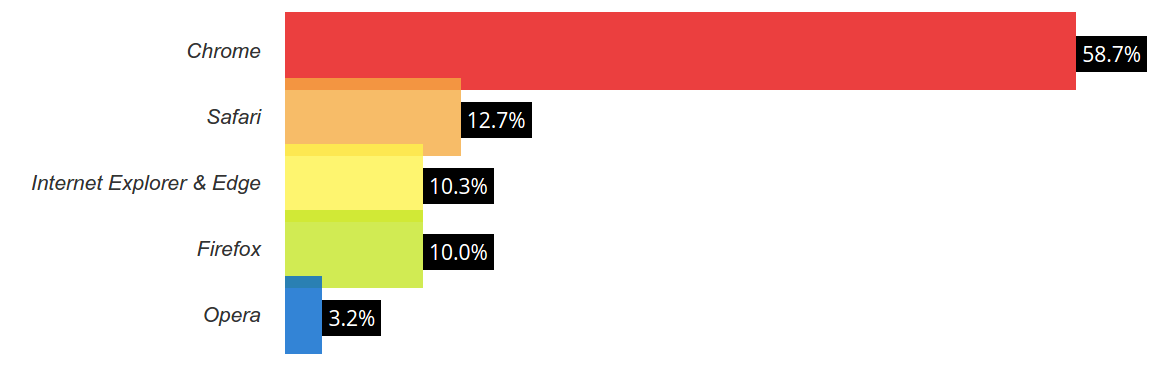
\includegraphics[scale=0.3]{img/browser_2016.png}
  \caption{Die fünf meistgenutzten Browser im Mai 2016}\label{fig:browser-may-2016}
\end{figure}

\subsection{Interoperabilität}
\label{sec:Interoperabilität_Analyse}
Auch bei den Webapplikationen ist es wichtig, bereits existente Frameworks und Problemlösungen nutzen zu können. Dementsprechend müssen externe JavaScript und CSS Bibliotheken ohne große Probleme eingebettet werden können. Dies kann bequem über die vorhandenen HTML-Tags und ihre Attribute gemacht werden.


\subsection{Asynchrones Laden}
\label{sec:Asynchrones Laden}
Nicht immer ist es sinnvoll, sämtliche Daten die auf einer Webseite angezeigt werden auch direkt an den Nutzer zu schicken. Sind beispielsweise große Datenmengen erst nach mehrmaligem Scrollen durch den Nutzer sichtbar, kann es ausreichen die Daten asynchron nachzuladen, sobald der Viewport, also der für den Nutzer sichtbare Bereich, sich diesem Inhalt nähert. Auf diese Weise kann der Server entlastet und die Ladezeit für den Nutzer verringert werden. Dieses Verhalten wird „Lazy Load“ genannt (XY). Besonders wenn davon auszugehen ist, dass der Nutzer nur einen sehr eingeschränkten Viewport oder eine schlechte Internetverbindung hat, bietet sich das asynchrone nachladen von Daten an.


\subsection{Dateigröße}
\label{sec:Dateigroesse}
Die Größe einer Datei wirkt sich auf die Dauer der Übertragungszeit aus. Ist die Datei groß, müssen entsprechend viele Informationen vom Server auf den Client des Nutzers übertragen werden, um die Webseite ansprechend darzustellen. Die Dateigröße kann mit einfachen Mitteln verringert werden. Beispielsweise können alle nicht unbeding notwendigen Zeichen aus der Datei entfernt werden. Dazu gehören Zeichen wie „Leerzeichen“ (Whitespaces) oder Zeilenumbrüche. Doch auch die Verkürzung von Variablen ist denkbar. Anstelle von „EinZiemlichLangesWort“ reicht beispielsweise „a“ komplett aus, muss dann natürlich an jeder anderen Stelle auch ersetzt werden. Hierzu bedarf es Algorithmen, welche die Nutzung von Variablen genau untersuchen und Fehler durch Ersetzungen vermeiden.



\section{Empirische Analyse}
\label{sec:Empirische Analyse}
\subsection{Versuchsaufbau}
\label{sec:Versuchsaufbau}
Abbildung XY: Zeigt die Kommunikation zwischen Client und Webserver
Die Abbildung XY zeigt die geplante Kommunikation zwischen dem Client, also dem Nutzer und dem Webserver.
In Schritt 1 fordert der Nutzer die Webseite an, erzeugt also einen Request. Dieser geht in Schritt 2 bei dem Webserver ein und wird verarbeitet. Abhängig von der angeforderten URL erzeugt der Webserver dann eine Antwort, mit allen zu sendenden Informationen und dem dazugehörigen HTML, CSS und JavaScript Code. Im nächsten Schritt 3 werden diese Daten zurück an den Client gesendet. Der Client nimmt die Daten entgegen, wie in Schritt 4 beschrieben. Des Weiteren macht der Client die Daten entsprechend sichtbar, so dass der Nutzer nun eine vollständige Präsentation der Webseite sieht. Schritt 5 beschreibt die mögliche Interaktion des Nutzers mit dem ihm präsentierten Dokument. Jede Interaktion führt zu einer Reaktion durch Javascript, oder erzeugt einen neuen Request an den Server, womit wieder bei Schritt 1 begonnen wird. Das Einbinden von CSS und JS aus externen Quellen wird durch Schritt 6 verbildlicht.
Die gesamte Applikation wird von einem fertigen Template, programmiert in HTML, CSS und JavaScript in die Programmiersprache Elm überführt, insofern möglich. Der daraus entstehende Elm-Quellcode wird dann mit dem Elm-Compiler kompiliert zu JavaScript.
Um ein generelles Verständnis der Programmiersprache Elm zu bekommen, dient die Dokumentation auf http://elm-lang.org/docs als Hilfestellung. Dort besteht die Möglichkeit sich mit den grundlegenden Konzepten vertiefend auseinanderzusetzen und diese zu erlernen.
Die zugrunde liegende Elm-Version ist 0.17 und wird unter Ubuntu 14.04 64bit installiert. Als Editor wird Atom mit mehreren Elm-Plugins verwendet, so dass der geschriebene Code automatisch beim Speichern formatiert und durch den Compiler auf Fehler überprüft wird.
Lauffähig wird die geschrieben Applikation mit dem Elm-Compiler $elm-make$ gemacht und dann mit Google Chrome Version 50 getestet.

\subsection{Hypothesen und Vermutungen}
\label{sec:Hypothesen und Vermutungen}
TODO: Aufzählung importieren

\subsection{Versuchsdurchführung}
\label{sec:Versuchsdurchführung}
\subsubsection{Installation}
\label{sec:Installation}
Zunächst einmal ist es notwendig, Elm und die dazugehörigen Komponenten zu installieren. Im folgenden wird die Installation unter Ubuntu 14.04 64bit erklärt.
Elm wird über den NPM verbreitet. Um diesen zu installieren, sind folgende Kommandos auf der Kommandozeile auszuführen:

\begin{lstlisting}[language=bash]
$ sudo apt-get update
$ sudo apt-get install nodejs
$ sudo apt-get install npm
\end{lstlisting}

Dadurch wird das NodeJs-Paket installiert und ausführbar gemacht. Aufgrund der Tatsache, dass viele Pakete nicht $nodejs$, sondern $node$ als ausführbare Datei erwarten, wird noch sicherheitshalber ein Symlink erstellt.

\begin{lstlisting}[language=bash]
$ sudo ln -s /usr/bin/nodejs /usr/bin/node
\end{lstlisting}
Anschließend sollte überprüft werden, ob die Installation erfolgreich war und sowohl NodeJS, wie auch NPM verfügbar sind. Das Kommando \begin{lstlisting}[language=bash]
$ node -v && npm -v
\end{lstlisting}
liefert den Output, wie er in Abbildung XY zu sehen ist. Elm kann nun über die Paketverwaltung NPM mit dem Kommando 
$npm\,install\,-g\,elm$ installiert werden. Das $-g$ -Flag installiert die neueste Elm-Version global für alle Projekte auf dem System. Entfernt man es, wird die Zielversion nur für den aktuellen Ordner zugänglich gemacht. Um die hier behandelte Version 0.17 zu installieren, ist der Zusatz $@0.17$ direkt hinter dem globalen Flag notwendig.\\
Elm ist nun vollständig installiert und kann genutzt werden. Die Entwicklung in Atom wird unterstützt durch die Pakete $elm-format$\\ (https://github.com/triforkse/atom-elm-format), $language-elm$\\ (https://atom.io/packages/language-elm) und {$linter-elm-make$}\\ (https://atom.io/packages/linter-elm-make). Mit Hilfe dieser Pakete wird der Code automatisch beim speichern dem Style-Guide entsprechend formatiert, eventuelle Fehler bei der Kompilierung direkt im Editor sichtbar gemacht und der Code syntaktisch gefärbt, sowie Vorschläge zur Vervollständigung des geschriebenen Quellcodes gemacht. Da die Pakete ständig aktualisiert und verändert werden, wird an dieser Stelle von einer detaillierten Beschreibung zur Installation abgesehen und auf die Dokumentationen der einzelnen Pakete verwiesen (elm-lang.org).
Damit die geschriebene Applikation letztendlich im Browser aufrufen zu können, muss die Elm-Applikation zunächst in der HTML-Datei aufgerufen und initialisiert werden. Dabei gibt es mehrere Möglichkeiten. Es ist sinnvoll hierbei zwischen vollautomatischem, sowie manuellem Grundaufbau zu unterschieden.
\subsubsection{Grundaufbau}
\label{sec:Grundaufbau}

1) Vollautomatisch – Elm-reactor\\
Mit Hilfe des $elm-reactor$, einem mitgelieferten Tools um den erzeugten Elm-Code lauffähig zu machen und die Applikation debuggen zu können, kann der gesamte Prozess der Kompilierung und Konfiguration eines Webservers automatisiert werden. Dafür muss lediglich der Ordner in dem die Elm-Applikation abgelegt wurde geöffnet und der $elm-reactor$ gestartet werden. 
Der Code kann automatisch kompiliert und zusätzlich eine $elm.html$ Datei erzeugt werden. Diese Datei wird dann mit dem gesamten kompilierten Elm-Code bestückt. Außerdem wird automatisch Code erzeugt, der den kompilierten JavaScript-Code ausführt. Für den Entwickler bedeutet dies, dass nur noch die erzeugten Dateien weitergegeben werden müssen. Die gesamte geschriebene Applikation ist darin enthalten und kann mit jedem Browser über die URL $http://localhost:8000/$ geöffnet werden, ohne die Notwendigkeit eines zusätzlichen Webservers. Die Abbildung ~\ref{fig:elm-reactor}) zeigt den laufenden Webserver.
\begin{figure}[hb]
\centering
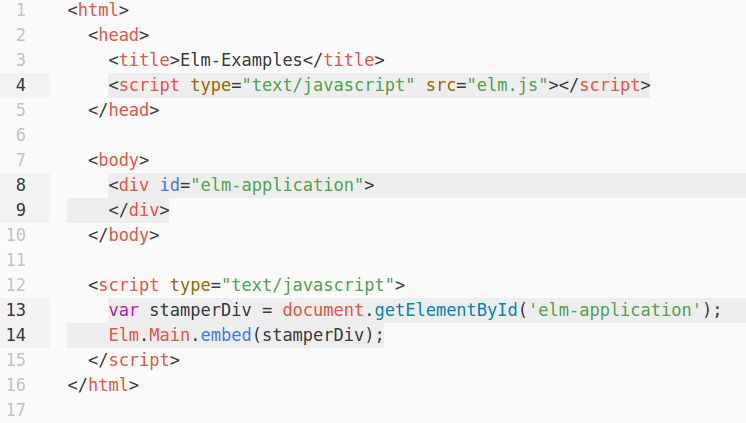
\includegraphics[scale=0.4]{img/elm-make_include_in_index.png}
\caption{Grundgerüst eines HTML-Dokumentes, um die Elm Applikation zu laden}\label{fig:html-boilerplate}
\end{figure}
\begin{figure}[t]
\centering
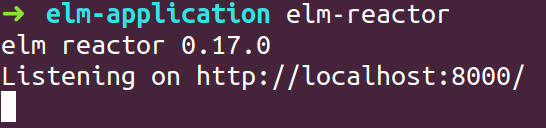
\includegraphics[scale=0.4]{img/elm-reactor.png}
\caption{Der gestartete Elm-Webserver}\label{fig:elm-reactor}
\end{figure}
Überlässt man dem Compiler das Einbinden der erzeugten JavaScript-Datei, so ist die gesamte Elm-Applikation im Vordergrund. Das ist nicht immer wünschenswert oder gar praktikabel. Einerseits, da externe Quellen für CSS und JavaScript über natives Elm nicht reibungslos geladen werden können, andererseits weil nicht immer der gesamte darzustellende HTML-Code nur in Elm geschrieben wurde. Dementsprechend gibt es auch die Möglichkeit, eine HTML-Datei als Gerüst zu erzeugen, in die gezielt der JavaScript-Code der Elm-Applikation injiziert wird. Das Gerüst ist vollständig wie eine klassische HTML-Datei aufgebaut. Abbildung~\ref{fig:html-boilerplate} zeigt das Grundgerüst des HTML-Dokumentes. Codezeile $4$ bindet die kompilierte Elm-Datei. Der \ac{DOM}-Knoten in welchen die Applikation injiziert wird, ist in Zeile $8$ definiert. Das injizieren der Applikation geschieht in den Zeilen $13$ bis $14$ und erhält als Parameter den zuvor erwähnten \ac{DOM}-Knoten. Um die Elm-Applikation einfügen zu können, muss die Elm-Datei vorher in der Kommandozeile kompiliert werden mit dem Kommando \colorbox{lightgray}{\lstinline{elm-make Datei.elm --output=elm.js}}.
Bei dieser Art der Initialisierung kann nun noch zwischen drei weiteren Darstellungen unterschieden werden:
\begin{enumerate}
\item$fullscreen$: Der erzeugte Code der Applikation wird in den Body-Tag einer HTML-Datei geladen und überschreibt den sonstigen HTML-Code.

\item$embed$: Der erzeugte Code der Applikation wird in den übergebenen DOM-Knoten geladen.

\item$worker$: Initialisiert die Applikation ohne grafische Benutzeroberfläche.
\end{enumerate}
Der Vorteil bei Version 2, so wie es auch in der Abbildung~\ref{fig:html-boilerplate} realisiert wurde, ist, dass auch nur kleine Teile der gesamten Applikation in Elm implementiert werden können. Überlegt man ein bestehendes, möglicherweise komplexes Projekt zu portieren, genügt es kleinere Teile Stück für Stück zu portieren. Es muss nicht befürchtet werden, große Teile der bestehenden Applikation während der Portierung nutzlos zu machen. Ein weiterer Vorteil ist, dass externes CSS und JavaScript in dem \ac{HTML}-Dokument über die \ac{HTML}-eigenen $<script>$-Tags geladen werden kann.
Zusätzlich zum Grundgerüst der $elm.html$ muss nun noch das Grundgerüst der eigentlichen Elm-App erstellt werden. Wie im Kapitel \nameref{sec:grundlagen} beschrieben, ist Elm nach einem \ac{MVU}-Konzept aufgebaut. Entsprechend sind das die unbedingt notwendigen Funktionen, die es zu realisieren gilt. Das standardmäßig mitgelieferte Paket $elm-lang/html$ liefert die sogenannten $Html.App$-Funktionen. Diese kümmern sich um die Bereitstellung und Auslieferung der Applikation, so dass sich Entwickler ganz auf die eigentliche Programmierung konzentrieren können. Dabei variieren stets die Übergabeparameter, wodurch die Applikation leicht erweitert und komplexer werden kann, ohne Neulinge direkt abzuschrecken. So verlangt die Funktion $Html.App.beginnerProgram$ nur die bekannten Funktionen $model$, $view$ und $update$. Hierbei können jedoch keine asynchronen Funktionen wie \ac{HTTP}-Requests genutzt werden.
Dafür gibt es die erweiterte Funktion $Html.App.program$, die als vierten Übergabeparameter sogenannte $subscriptions$ erwartet. $Subscriptions$ werden für die Kommunikation zwischen Elm und Javascript, sowie die Verbindung zu Websockets genutzt.
Die dritte und letzte Möglichkeit ist die Funktion $Html.App.programWithFlags$. Hierbei wird die Übergabe eines initialen $Models$ an die Elm-Applikation ermöglicht, um den Zustand der Applikation dynamisch setzen zu können.
\begin{figure}[ht]
\centering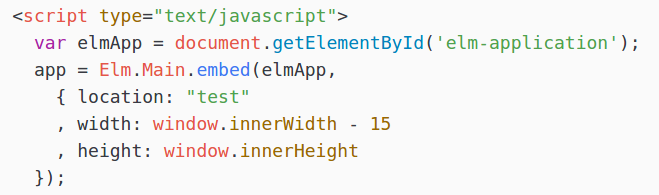
\includegraphics[scale=0.6]{img/programWithFlags_pass_data.png}
\caption{Eine beispielhafte Initialisierung der Elm-Applikation mit übergebenen Werten}\label{fig:programWithFlags}
\end{figure}
Abbildung~\ref{fig:programWithFlags} zeigt das Grundgerüst einer Elm-Applikation mit der Implementierung der Funktion $Html.App.programWithFlags$. Die $main$ Funktion erstellt dabei die eigentliche Applikation, während die Funktionen $model$, $view$ und $update$ jeweils den Zustand und die gewünschte Darstellung der Applikation beschreiben, sowie vorgeben, wie mit der Interaktion durch den Benutzer umgegangen wird. Die Funktion $subscription$ gibt in diesem Stand noch keinerlei Daten weiter und stellt eine Dummy-Funktion dar. $initialModel$ erzeugt beim Aufruf ein Model mit initialen Werten, die dem Model ($type\,alias\,Model$) entsprechen müssen. Durch das Grundgerüst der $elm.html$ und $Main.elm$-Datei kann die Applikation nun schrittweise erweitert und Funktionen hinzugefügt werden. Zuletzt wird der erzeugte Code modularisiert.

\subsubsection{Konstruktion des Views}
\label{sec:Konstruktion des Views}
TODO: Rewrite:
\begin{enumerate}
	\item Konstruktion des Views
	\subitem{-} Import der HTML-Bibliothek
	\subitem{-} Aufruf der HTML-Funktion
	\subitem{-} Signatur der HTML-Funktion
	\subitem{-} Verschachtelung verschiedener Aufrufe
	\subitem{-} Unterschied HTML vs. Elm
		\subsubitem{-} HTML: Öffnende + schließende Tags (Fehleranfällig, unübersichtlich, schachtelbar in einer Zeile)
		\subsubitem{-} Elm: Einrückung (indention sensitive)
	\subitem{-} Mathematisch ausdrücken, dass Elm-Code im Gegensatz zu HTML 'kürzer' ist
	\subitem{-} Fehleranfälligkeit von HTML klarstellen
\end{enumerate}


Lorem ipsum dolor sit amet, consetetur sadipscing elitr, sed diam nonumy eirmod tempor invidunt ut labore et dolore magna aliquyam erat, sed diam voluptua. At vero eos et accusam et justo duo dolores et ea rebum. Stet clita kasd gubergren, no sea takimata sanctus est Lorem ipsum dolor sit amet. Lorem ipsum dolor sit amet, consetetur sadipscing elitr, sed diam nonumy eirmod tempor invidunt ut labore et dolore magna aliquyam erat, sed diam voluptua. At vero eos et accusam et justo duo dolores et ea rebum. Stet clita kasd gubergren, no sea takimata sanctus est Lorem ipsum dolor sit amet. Lorem ipsum dolor sit amet, consetetur sadipscing elitr, sed diam nonumy eirmod tempor invidunt ut labore et dolore magna aliquyam erat, sed diam voluptua. At vero eos et accusam et justo duo dolores et ea rebum. Stet clita kasd gubergren, no sea takimata sanctus est Lorem ipsum dolor sit amet.   

Duis autem vel eum iriure dolor in hendrerit in vulputate velit esse molestie consequat, vel illum dolore eu feugiat nulla facilisis at vero eros et accumsan et iusto odio dignissim qui blandit praesent luptatum zzril delenit augue duis dolore te feugait nulla facilisi. Lorem ipsum dolor sit amet, consectetuer adipiscing elit, sed diam nonummy nibh euismod tincidunt ut laoreet dolore magna aliquam erat volutpat.   

Ut wisi enim ad minim veniam, quis nostrud exerci tation ullamcorper suscipit lobortis nisl ut aliquip ex ea commodo consequat. Duis autem vel eum iriure dolor in hendrerit in vulputate velit esse molestie consequat, vel illum dolore eu feugiat nulla facilisis at vero eros et accumsan et iusto odio dignissim qui blandit praesent luptatum zzril delenit augue duis dolore te feugait nulla facilisi.   

Nam liber tempor cum soluta nobis eleifend option congue nihil imperdiet doming id quod mazim placerat facer possim assum. Lorem ipsum dolor sit amet, consectetuer adipiscing elit, sed diam nonummy nibh euismod tincidunt ut laoreet dolore magna aliquam erat volutpat. Ut wisi enim ad minim veniam, quis nostrud exerci tation ullamcorper suscipit lobortis nisl ut aliquip ex ea commodo consequat.   

Duis autem vel eum iriure dolor in hendrerit in vulputate velit esse molestie consequat, vel illum dolore eu feugiat nulla facilisis.   

At vero eos et accusam et justo duo dolores et ea rebum. Stet clita kasd gubergren, no sea takimata sanctus est Lorem ipsum dolor sit amet. Lorem ipsum dolor sit amet, consetetur sadipscing elitr, sed diam nonumy eirmod tempor invidunt ut labore et dolore magna aliquyam erat, sed diam voluptua. At vero eos et accusam et justo duo dolores et ea rebum. Stet clita kasd gubergren, no sea takimata sanctus est Lorem ipsum dolor sit amet. Lorem ipsum dolor sit amet, consetetur sadipscing elitr, At accusam aliquyam diam diam dolore dolores duo eirmod eos erat, et nonumy sed tempor et et invidunt justo labore Stet clita ea et gubergren, kasd magna no rebum. sanctus sea sed takimata ut vero voluptua. est Lorem ipsum dolor sit amet. Lorem ipsum dolor sit amet, consetetur sadipscing elitr, sed diam nonumy eirmod tempor invidunt ut labore et dolore magna aliquyam erat.   

Consetetur sadipscing elitr, sed diam nonumy eirmod tempor invidunt ut labore et dolore magna aliquyam erat, sed diam voluptua. At vero eos et accusam et justo duo dolores et ea rebum. Stet clita kasd gubergren, no sea takimata sanctus est Lorem ipsum dolor sit amet. Lorem ipsum dolor sit amet, consetetur sadipscing elitr, sed diam nonumy eirmod tempor invidunt ut labore et dolore magna aliquyam erat, sed diam voluptua. At vero eos et accusam et justo duo dolores et ea rebum. Stet clita kasd gubergren, no sea takimata sanctus est Lorem ipsum dolor sit amet. Lorem ipsum dolor sit amet, consetetur sadipscing elitr, sed diam nonumy eirmod tempor invidunt ut labore et dolore magna aliquyam erat, sed diam voluptua. At vero eos et accusam et justo duo dolores et ea rebum. Stet clita kasd gubergren, no sea takimata sanctus.   

\iffalse
Das erste sichtbare Modul der fertigen SPA ist die Navigationsleiste. Sie soll dem Nutzer die Möglichkeit bieten schnell und einfach einen Überblick über die vorhandenen Themen auf der Webseite zu erhalten und direkt mit einem Klick auf den Reiter zu einem Thema zu springen. Damit die Navigation während des gesamten Besuches möglich ist, soll die Navigationsleiste `fixed` sein, also am oberen Bildschirmrand fest verankert bleiben und mit scrollen.
Jedes Modul der dargestellten Seite besteht aus HTML-Code. Folglich müssen HTML-Tags mit Elm generiert werden. Seit dem neuesten Release von Elm (Version 0.17) wurden einige Pakete die sich für die Webentwicklung nutzen lassen zusammengeführt in das Paket `elm-lang/html`. Es erlaubt die Erzeugung von HTML und CSS mit nativem Elm-Code. In Elm können HTML-Tags mit bereitgestellten Funktionen aus diesem Paket erzeugt werden. Ein HTML `div`-Tag wird mit der gleichnamigen Funktion `div` erzeugt. Die Funktion erwartet zusätzlich zwei Argumente. Einerseits eine Liste von HTML-Attributen wie `class`, `id` oder `href`, andererseits eine Liste von weiteren HTML-Tags, insofern Code geschachtelt wird. Die Signatur für diese Funktion lautet wie folgt:
`div (List Html.Attribute msg) (List Html.Html msg)`
Entsprechend dieser Signatur wird in Abbildung XY gezeigt, wie die `div`-Funktion in Elm nach der Kompilierung in HTML dargestellt wird.
Nicht nur die Erstellung eines HTML-Tags, sondern auch die Zuweisung von Attributen ist in Elm eine Funktion. So sieht man in Abbildung XY ebenso, wie eine Klasse (`class`) und ID einem Element hinzugefügt wird. Da in Elm sämtliche Funktionen „pure functions“, also reine Funktionen sind, hat der Entwickler die Sicherheit, dass das Resultat der Funktion immer gleich bleibt.
Des Weiteren ist es möglich die HTML-Elemente nativ in Elm mit CSS-Styling zu versehen. Dafür wird die gleichnamige Funktion `style` aus dem Paket genutzt. Auch diese Funktion erwartet eine Liste von Argumenten, jeweils mit einem Schlüssel (hier: CSS-Eigenschaft) und dem dazugehörigen Wert. Zur Zeit ist es nicht problemlos möchlich nativ in Elm eine externe CSS-Datei zu integrieren. Corey Trampe (https://gist.github.com/coreytrampe/a120fac4959db7852c0f) hat eine Möglichkeit gefunden, jedoch wird bei dieser Lösung die Seite zunächst ohne jegliches Styling dargestellt, während ein asynchroner Request die externe CSS-Datei lädt. Sobald dieser Vorgang abgeschlossen ist, wird das heruntergeladene Styling angewandt. Der zeitliche Abstand zwischen initialem Laden und der Anwendung des Styles hat ein sichtbares „flackern“ zur Folge, wodurch eine Nutzung in einem fertigen System entfällt. Alternativ werden alle zu ladenden CSS-Dateien im HTML-Grundgerüst über den HTML-Tag `link` eingebunden.
\fi

\subsubsection{Überführung des Views}
\label{sec:Überführung des Views}
Für die Darstellung einer SPA wird ein fertiges und kostenloses Theme von `startbootstrap.com` verwendet. Im Zuge dessen werden alle verfügbaren Dateien heruntergeladen und die zuvor erstellten Dateien `elm.html` und `Main.elm` in denselben Ordner verschoben.
Das Grundgerüst der `elm.html` muss nun in die `index.html` überführt werden, so dass die Elm-Applikation weiterhin in den vorhandenen HTML-Code injiziert wird.
Zunächst einmal muss der HTML-Code des Themes in ausführbaren Elm-Code umgeschrieben werden, damit Elm Zugriff auf den kompletten `view` bekommt. Nur so kann Elm die Interaktion des Benutzers mit den HTML-Elementen abfangen und entsprechend darauf reagieren. Um nicht den kompletten HTML-Code der `index.html` per Hand in Elm-Code überführen zu müssen, wird das Tool `html-to-elm` genutzt (http://mbylstra.github.io/html-to-elm/). Dieses Online-Tool erlaubt es HTML5-konformen Code in lauffähigen Elm-Code zu überführen. Der erzeugte Elm-Code wird dann in der `Main.elm`-Datei von der `view`-Funktion zurückgegeben., muss also entsprechend dort eingefügt werden.
Um Modularität zu gewährleisten, wird jede Sektion der SPA, wie zum Beispiel die Navigation, die Team-Sektion oder der Footer im ersten Schritt in eine eigene Funktion ausgelagert. Jede dieser Funktionen wird dann in der `view`-Funktion aufgerufen und ergibt am Ende die gesamte Webseite. Auf diese Weise können die einzelnen Teile der SPA unabhängig voneinander modifiziert und auf Korrektheit überprüft werden. Im nächsten Schritt wird der gesamte View-Code modularisiert.

\subsubsection{Modularisierung}
\label{sec:Modularisierung}
Damit ein Entwickler den Überblick über den vorhandenen Quellcode behält ist es sinnvoll einzelne Teile der Applikation in mehrere Dateien und Ordner zu verschieben. Eine solche Strukturierung hilft dabei die womöglich fehlerbehafteten Teile der Applikation zu finden und beispielsweise die Programmlogik noch deutlicher von der Applikationsdarstellung zu trennen. Dabei werden die einzelnen Funktionen des Views, also die für die Darstellung verantwortlichen Programmteile, ausgelagert in eigene Module. Dasselbe wird für die `Update` und `Model` relevanten Funktionen durchgeführt. Die notwendigen Funktionen eines jeden Moduls werden dann im Gegenzug vom Hauptmodul importiert und an den entsprechenden Stellen aufgerufen.\\\\
\noindent\textbf{View}\\
Jede bisherige Funktion aus dem View wird in den Ordner `View` verschoben und als gleichnamiges Modul benannt. Jedes Modul bekommt dabei den Namen des Ordners in dem es zu finden ist, gefolgt vom Namen des Views, dass es darstellt. Das für die Navigation verantwortliche Modul wird  entsprechend mit `module View.Navigation exposing (view)` initialisiert und gibt die Funktion `view` an jedes importierende Modul frei.
Dieser Schritt dient lediglich der besseren Strukturierung des Quellcodes und der Vereinfachung für den Entwickler. Abbildung XY zeigt die Haupt-`view`-Funktion nachdem sämtliche Teile des `View`s modularisiert und entsprechend importiert wurden.\\\\
\noindent\textbf{Update}\\
Auch die Programmlogik kann modularisiert werden und wird dafür in den Unterordner $Update$ verschoben. Hierfür werden sämtliche Typdeklarationen ($Msg$), sowie die dazugehörige Funktion $update$ in das neue Modul `Update.Update` verschoben und auch die notwendigen Pakete hinzugefügt. Von außen kann auf das $Update$-Modul, nachdem es importiert wurde, mit dem Namespace $Update$ zugegriffen werden.\\\\
\textbf{Model}\\
Letztlich wird noch das $model$, das sämtliche Daten die den Status der Applikation beschreiben enthält, in ein eigenes Modul im Unterordner $Model$ überführt. Die Einbindung dieses Moduls funktioniert analog zur Modularisierung von $Update$ und $View$.
Mit Hilfe dieser Modularisierung wird das angestrebte \ac{MVU}-Konzept von Elm besonders deutlich.

\subsubsection{Asynchrones Laden}
\label{sec:Asynchrones Laden - Analyse}
Das fertige Template bietet die Möglichkeit auf einen Portfoliobeitrag zu klicken. Durch diesen Klick wird ein Modal geöffnet, in das weitere Informationen dargestellt werden. Üblicherweise werden diese zusätzlichen Informationen in einer \ac{SPA} nachgeladen, um das initiale Laden der Applikation zu verkürzen und nur wirklich notwendige Daten anzuzeigen. Die bestehende Elm-Applikation wird nun um das Feature des asynchronen Ladens von Informationen erweitert.
Zunächst muss das $model$ erweitert und angepasst werden, da dies die einzige Möglichkeit in einer Elm-Applikation ist, Daten beziehungweise den Status der Applikation zu speichern. Das `model` bekommt entsprechend ein weiteres Feld `async-content : String`.
Bei einem Klick auf eines der Portfoliobeiträge soll entsprechend das Modal geöffnet und ein Titel präsentiert werden. In diesem Beispiel wird über eine externe API ein zufälliger String angefordert, vom Server generiert und dann an die Elm-Applikation zurückgegeben. Ebenso wäre es möglich einen Server für das Backend zu erstellen, auf dem eine Datenbank läuft, so dass Daten asynchron angefordert werden können. In diesem Fall ist es jedoch nicht notwendig ein zusätzliches Backend zu konfigurieren.
Ein solcher asynchroner Request stellt im Grunde eine Verletzung des Konzeptes von Elm dar, dass es keinerlei Seiteneffekte gibt. Da nicht bekannt ist, wann der Request endet und welchen Status die Antwort besitzt (Failed, Success, ..?), ist zunächst nicht vorhersehbar, wie der Status der Applikation nach dem Request aussehen wird. Um dieses Problem zu vermeiden, ist es notwendig alle möglichen Fälle , also den Fall einer erfolgreichen, sowie fehlerhaften Übertragung, zu behandeln. Auf diese Weise ist gewährleistet, dass die Applikation sich nicht plötzlich in einem nicht definierten Zustand befindet.
Einen asynchronen Request in Elm auszuführen bedarf mindestens zweier zusätzlicher Funktionen und der Importierung der Bibliotheken $Http$, $Json.Decode$ und $Task$. Des Weiteren muss der Klick auf das Portfolio-Element abgefangen werden. Dafür gibt es die $onClick$ Funktion aus der $Html.Events$-Bibliothek. Sie bekommt die auszuführende Funktion als Parameter, sieht also wie folgt aus: `onClick Update.GetRandomString`. Die möglichen `Types` von eingehenden Nachrichten (`Msg`/Klicks) wird erweitert um `GetRandomString`, sowie auch die `update`-Funktion um diesen Typ erweitert werden muss. Der entsprechende `update`-Fall `GetRandomString` gibt dann das `model`, sowie einen Effekt `fetchAsync` zurück. Die Definition dieses Effektes ist der Grund, weshalb hier von einem `managed Effect` die Rede ist und der Seiteneffekt kontrolliert verläuft. `fetchAsync` ist hierbei erneut eine Funktion, die eine Nachricht (`Msg`) an die `update`-Funktion mit dem Ergebnis des Requests zurückgibt . Elm führt den Request in Form eines `Task` aus und erwartet eine Funktion für den Fall einer erfolgreichen Übertragung, sowie eine Funktion für jeglichen Fehlerfall. In beiden Fällen wird die entsprechende Funktion ausgeführt und an die `update`-Funktion zurückgegeben. Hier wird, insofern notwendig, ein neues `model` mit veränderten Werten erzeugt und letztlich das Ergebnis auf dem Bildschirm des Nutzers sichtbar gemacht.\\
TODO: Allgemeiner beschreiben. Bei Bezug auf den Anwendungsfall, Abbildung einfügen.

\subsection{Beobachtungen}
\label{sec:Beobachtungen}
Während der Entwicklung der Elm-Applikation kam es zu unvorhergesehenen Problemen, sowie teilweisen Erkentnissen. Diese Beobachtungen werden im folgenden stichpunktartig zusammengefasst und anschließend erläutert.
\begin{enumerate}[label*=\arabic*.]

\item Externes \ac{CSS} kann nicht nativ über Elm geladen werden
	\begin{enumerate}[label*=\arabic*.]
		\item Inline-\ac{CSS} muss manuell mehrfach abgeändert werden
		\item Keine Schachtelung möglich
		\item Browser kann inline-\ac{CSS} nicht zwischenspeichern
	\end{enumerate}
\item HTML-Code ist in Elm kürzer
	\begin{enumerate}[label*=\arabic*.]
		\item \ac{HTML}-Code benötigt in Elm keine schließenden Klammern. Anders als \ac{HTML} arbeitet Elm mit Einrückungen. Die gleichnamigen Funktionen um ein \ac{HTML}-Element zu erzeugen benötigen dementsprechend lediglich den Funktionsaufruf, gefolgt von den zwei Argumenten. Das bedeutet, dass nativer Code in Elm kürzer und weniger anfällig für Flüchtigkeitsfehler wie beispielsweise das Schließen eines Tags ist. Der Entwickler wird weniger syntaktische Fehler machen.
	\end{enumerate}
\item Vertikale und horizentrale Zentrierung eines Elementes
	\begin{enumerate}[label*=\arabic*.]
		\item Obwohl Elm ein Paket für genau dieses Anwendungsgebiet besitzt, ist die Anwendung dennoch weder simpel, noch voll funktionsfähig. Es bedarf einiger Transformationen der Elemente, um sie in nutzbare, validen \ac{HTML}-Code zu formatieren. Zuletzt trifft der Entwickler auf die Problematik, zusätzlich noch die explizite Größe des Fensters mit einbeziehen zu wollen, so dass das Element den gesamten Bildschirm ausfüllt und einen zentrierten Text beinhaltet. Die Fenstergröße zu ermitteln stellt ein größeres Hindernis dar, als zunächst erwartet. Die Möglichkeiten sind hier, halbwegs dynamisch die Fenstergröße bei der Initiierung der Elm-Applikation an diese weiter zureichen, oder über Ports abzufangen, wenn sich die Fenstergröße geändert hat. Die erste Lösung hilft nur, wenn die Größe des Fensters nicht weiter verändert wird. Dies kann jedoch nicht gewährleistet werden, wodurch die Lösung entfällt. Die zweite Lösung hingegen erzeugt eine zusätzliche Abhängigkeit zwischen Elm und externem Javascript. Zuletzt bleibt noch die altbekannte Möglichkeit mittels \ac{CSS} den Text in einem Element beidseitig zu zentrieren. Hierfür kann das externe \ac{CSS}-Framework Flexbox zuhilfe gezogen werden. Flexbox kümmert sich um die horizontale und vertikale Platzierung von Elementen, ohne auf die \ac{CSS}-Eigenschaft „float“ zurückgreifen zu müssen, die gerade bei tief verschachtelten Elementen Probleme verursacht.
		
		\item Das Paket `elm-lang/window` stellt eine Funktion `resize` zur Verfügung, die bei jeder Veränderung der Fensterdimensionen über eine sogenannte `subscription` in Elm einen Aufruf der `update` Funktion auslöst, an jene die neuen Fensterdimensionen (X, Y) weitergereicht werden.
	\end{enumerate}

\item Elm-Compiler
	\begin{enumerate}[label*=\arabic*.]
		\item Kompiliert abhängig von der Tiefe der Elemente
		\begin{enumerate}[label*=\arabic*.]
			\item Entwickler muss lesbaren Code erzeugen, da Elm sensitiv auf Tabs reagiert (vs HTML: $<div><span></span></div>$ wo unendliches verschachteln auch in einer Zeile möglich ist)
		\end{enumerate}
	\end{enumerate}

\item TODO:
	\begin{enumerate}[label*=\arabic*.]
		\item Fehlende Beispiele importieren
		\item Umschreiben der Beispiele
	\end{enumerate}
\end{enumerate}



\subsection{Auswertung}
\label{sec:Auswertung}
\begin{table}[h]
\centering
\begin{tabular}{ | l | c | }
	\hline
	\textbf{Kriterium} & \textbf{Erfüllt}\\
	\hline
	1. Entwicklungsgeschwindigkeit & \\
	1.1 & \checkmark\\
	\hline
	2. Wartbarkeit & \\
	2.1  & \checkmark\\
	\hline
	3. Zuverlässigkeit & \\
	3.1  & \checkmark\\
	3.2  & \checkmark\\
	3.3  & \checkmark\\
	\hline
	4. Portabilität & \\
	4.1  & ausstehend\\
	\hline
	5. Effizienz & \\
	5.1  & \checkmark\\
	5.2  & ausstehend\\
	\hline
	6. Wiederverwendbarkeit & \\
	6.1  & \checkmark\\
	\hline
	7. Modularität & \\
	7.1  & \checkmark\\
	7.2  & \checkmark\\
	\hline
	8. Lesbarkeit & \\
	8.1  & \checkmark\\	
	\hline
	9. Dateigröße & \\
	9.1  & ausstehend\\
	\hline
	10. Interoperabilität & \\
	10.1  & \checkmark\\
	10.2  & Nein/Nur bedingt\\
	\hline
	11. Asynchrones Laden & \\
	11.1  & \checkmark\\
	\hline
\end{tabular}
\caption{Auswertung der Versuchskriterien}
\label{tab:Auswertungstabelle}
\end{table}
TODO: Importieren der schriftlichen Auswertung der Tabelle~\ref{tab:Auswertungstabelle}

 1.1. Elm hat leicht erlernbare Grundkonzepte, die adaptiert und erweiterbar sind, um Produktivität für die Entwickler zu gewährleisten.
 
 2.1. Elm Code kann mindestens kommentiert werden, wenn nicht sogar eine Funktion zur automatischen Generierung von Signaturen einer Funktion existiert
 --> Kommentare können mit `--` (single-line) oder `{- a comment - }` erstellt werden. Eine vollautomatische, explizite Erstellung der Signaturen besteht derzeit nicht. Der Compiler wird jedoch nach dem Kompiliervorgang einen Signaturvorschlag geben. Dieser Vorschlag ist auf einer niedrigeren Ebene, als es eine Deklaration wäre, ist jedoch ausreichend und wesentlich sinnvoller als eine Signatur komplett unberücksichtigt zu lassen. Beispiel: Abbildung XY ($compiler_sig_suggestion$ + $compiler_own_sig$)
 ```
 type alias Model = { counter: Int }
 increaseModel: Model -> Model
 increaseModel model =
     {model | counter = model.counter + 1}
 
 vs. Kompiliervorschlag
 type alias Model = { counter: Int }
 increaseModel: { a | counter : number } -> { a | counter : number }
 increaseModel model =
     {model | counter = model.counter + 1}
 ```
 
 3.1. Die Erweiterungen des Editors oder der Compiler warnt spätestens bei der Kompilierung, wenn nicht bereits während der Entwicklung vor syntaktischen Fehlern
 --> Syntaktische Fehler werden vom Compiler erkannt und ein Fehler angezeigt. Der Fehler wird unterstützt durch einen Hinweis auf die mögliche Fehlerquelle (Abbildung XY – $Compiler_syntax_error$). Die Fehlermeldung wird erst nach der Kompilierung eingeblendet.
 ```
 div [ id "elm-view" ]
         [ Navigation.view model
             Header.view
         , Services.view]
 ```
 
 3.2. Gibt es keine Fehlermeldungen, wird die Applikation ohne Laufzeitfehler funktionieren
 --> Aufgrund der Garantien, dass es keine Seiteneffekte gibt und alle Variablen unveränderlich sind, ist die Korrektheit syntaktische und semantische Korrektheit des Codes gewährleistet. Lediglich die logische Implementierung eines Algorithmus kann noch Fehler aufweisen, dies kann jedoch nicht von einem Compiler überprüft werden.
 3.3. Fehlermeldungen werden sehr spezifisch auf das eigentliche Problem hinweisen
 --> Wie in Abbildung iii.i zu sehen ist, gibt der Compiler nicht nur an, in welcher Zeile ein Fehler gefunden wurde, sondern liefert zusätzlich noch einen Hinweis, worin eine wahrscheinliche Fehlerquelle liegt. In diesem Beispiel weißt der Compiler auf das fehlende Komma als Fehlerquelle hin.
 
 4.1  1. Die SPA wird auf allen gängigen Browsern fehlerfrei dargestellt
 --> AUSSTEHEND
 
 5.1. Der Kompiliervorgang wird nur wenige Sekunden dauern, jedoch mehr Zeit in Anspruch nehmen, als die herkömmliche Entwicklung mit reinem HTML, CSS und JS
 --> Bei der herkömmlichen Entwicklung ist kein expliziter Kompiliervorgang notwendig, stattdessen übernimmt der Browser die Darstellung des übergebenen HTML, CSS und JS Quellcodes. Der Kompiliervorgang der Elm-Applikation dauert wie in Abbildung XY  zu sehen ist im Durchschnitt XY Sekunden. Es wurde 10x gemessen, der höchste und niedrigste Wert gestrichen und dann das arithmetische Mittel der verbleibenden 8 Messungen ermittelt.
 
 5.2  2. Die erzeugte Elm-Applikation ist deutlich schneller während der Laufzeit
 --> AUSSTEHEND (Abbildung - Performance - Evtl. neu?)
 
 6. 1. Codeteilen lassen sich problemlos auslagern und wiederverwenden
 --> Der komplette View wurde von einer großen Darstellung in mehrere Funktionen unterteilt und letztlich in ein eigenes Modul überführt. Analog dazu wurden auch das Model, sowie die Update-Funktion ausgelagert. Das einmalig definierte `Model` kann in sämtlichen Modulen wiederverwendet werden, auch die einzelnen Funktionen eines jeden Moduls finden erneut Verwendung, insofern gewünscht.
 
 7.1. Ausgelagerte Codeteile sind isoliert voneinander und als einzelnes Modul nutzbar
 --> Diese Eigenschaft ist gegeben.
 7.2. Module können Funktionen nach außen verbergen
 --> Jedes Modul kann mit dem Stichwort `expose` einzelne Funktionen nach außen hin zugänglich machen. Das importierende Modul wiederum kann einzelne Funktionen in den derzeitigen globalen `Scope` laden.
 
 8.1. Die automatische Formatierung des Elm-Codes macht diesen lesbarer und spart Zeit
 --> Fehler werden Dank der Formatierung schnell sichtbar.
 
 9.1. Die Dateigröße der Elm-Applikation wird kleiner als bei vergleichbaren Frameworks ausfallen
 --> Die kompilierte Elm-Applikation hat eine Größe von etwa 300kb. Allerdings kann diese Größe um etwa 60Prozent verringert werden, wenn der Code `minified` wird.
  
  10.1. Bestehende JS-Skripte können mit der Elm-Applikation interagieren oder funktionieren bereits einwandfrei
  --> Die Integration vorhandener JS-Skripte verlief problemlos. Benötigt ein externes Skript Daten von der Elm-Applikation, so kann mit Hilfe von `Ports` eine gesicherte Kommunikation in beide Richtungen stattfinden.
  
  10.2. Bestehender CSS-Code kann nativ in Elm eingebunden werden
  --> Das Einbinden von CSS Quellen ist derzeit nicht ohne Probleme nativ in Elm möglich. Es verursacht ein „flackern“ und ist nicht für den Gebrauch in einem fertigen System geeignet. CSS-Klassen und `inline-styling` sind jedoch nativ in Elm implementiert und erlauben ein Styling der Elemente. Externes CSS muss jedoch über das Grundgerüst der HTML-Datei eingebunden werden.
  
  11.1. Elm erlaubt asynchrone Requests ohne Seiteneffekte zu erzeugen
  --> Ein asynchroner Request stellt implizit einen Seiteneffekt dar, wird in Elm allerdings als gemanagter Seiteneffekt bezeichnet. In jedem Fall ist der Nutzer gezwungen eine Funktion bei einer fehlerhaften Übertragung zu übergeben, die dann die erwartenden Typen/Werte liefert.
  
  
  
  
  1. Installation sehr einfach
  1. externe Abhängigkeiten werden automatisch installiert
  2. Installation war schnell
  3. Erklärung zur Installation war deutlich
  2. Modularität möglich
  1. Jedes View-Element als eigenes Modul
  1. Paralleles arbeiten möglich
  2. Entwickler bekommen nur die notwendigen Informationen für das Interface
  3. Tools
  1. HTML2ELM sehr hilfreich
  1. Kleinere Fehler
  1. ' verursacht Fehler (Weiterfolgende Divs wurden vernachlässigt)
  2. required --> required '' (wants Bool, got String); novalidate same
  2. Elm-Compiler
  1. Fehler von HTML2ELM (2. Punkt) wurden sofort erkannt
  2. Fehlende Funktionen für HTML und CSS Attribute wurden in den Fehlermeldungen vorgeschlagen („Did you mean Html.Attributes.required?“ für „required true“)
  4. Erklärungen der Elm-Struktur in den Guides sehr gut

\chapter{Fazit}
\label{chap:fazit}
TODO:
\begin{enumerate}
	\item{Gegenüberstellung}
		\subitem{-} Was war das Ziel und der Wissensstand zu Beginn
		\subitem{-} Was waren die Erwartungen
		\subitem{-} Gab es unvorhergesehene Probleme? Wenn ja, welche?
		\subitem{-} Entsprach das Endergebnis (und der Weg dorthin) dem vorherigen Ziel?
	\item Aufzählung der maßgeblich wichtigen Punkte
	\item Résumé
		\subitem{-} Erfüllt Elm die Anforderungen der Webentwicklung?
		\subitem{-} Einstufung, für welche Anwender Elm geeignet ist
		\subitem{-} Aktuell (noch) bestehende Probleme, die es zu lösen gilt
\end{enumerate}

\chapter{Eidesstattliche Erklärung}
\label{sec:erklaerung}

Hiermit versichere ich, dass ich die vorliegende Arbeit selbstständig verfasst und ohne Benutzung
anderer als der angegebenen Hilfsmittel angefertigt, nur die angegebenen Quellen benutzt und die
in den benutzten Quellen wörtlich oder inhaltlich entnommenen Stellen als solche kenntlich
gemacht habe.
Die Arbeit hat in gleicher oder ähnlicher Form noch keiner anderen Prüfungsbehörde vorgelegen.\\
\\[1.5cm]
Kiel, den 07. Juli 2016
\\[2cm]
---------------------------------------------
\\
\enspace (Unterschrift)

\iffalse
\newpage
\addsec{Danksagungen}
\label{danksagungen}
Weit hinten, hinter den Wortbergen, fern der Länder Vokalien und Konsonantien leben die Blindtexte. Abgeschieden wohnen Sie in Buchstabhausen an der Küste des Semantik, eines großen Sprachozeans. Ein kleines Bächlein namens Duden fließt durch ihren Ort und versorgt sie mit den nötigen Regelialien. Es ist ein paradiesmatisches Land, in dem einem gebratene Satzteile in den Mund fliegen. Nicht einmal von der allmächtigen Interpunktion werden die Blindtexte beherrscht – ein geradezu unorthographisches Leben. Eines Tages aber beschloß eine kleine Zeile Blindtext, ihr Name war Lorem Ipsum, hinaus zu gehen in die weite Grammatik. Der große Oxmox riet ihr davon ab, da.
\fi


%Literaturverzeichnis
\bibliographystyle{unsrtdin}
\bibliography{Literatur}
TODO: Literatur hinzufügen + Referenzen + importieren

\end{document}
